
%%%%%%%%%%%%%%%%%%%%%%%%%%%%%%%%%%%%%%%%%%%%%%%%%%%%%%%

\documentclass{iitthesis}
%\documentclass[draft]{iitthesis}



\usepackage[dvips]{graphicx}    % This package is used for Figures
\usepackage{rotating}           % This package is used for landscape mode.
\usepackage{epsfig}
\usepackage{subfigure}          % These two packages, epsfig and subfigure, are used for creating subplots.
% Packages are explained in the Help document.
\usepackage{amsmath,amssymb,amsthm,mathtools,bbm,booktabs,array,tikz,pifont,comment,multirow,url,graphicx}
\usepackage{enumitem}
\usepackage[nodayofweek]{datetime}
\usepackage{color}
\input FJHDef.tex


\DeclareMathOperator{\Var}{Var}
\DeclareMathOperator{\INT}{INT}
\DeclareMathOperator{\APP}{APP}
\DeclareMathOperator{\lin}{lin}
\DeclareMathOperator{\up}{up}
\DeclareMathOperator{\lo}{lo}
\DeclareMathOperator{\fix}{fix}
\DeclareMathOperator{\err}{err}
\DeclareMathOperator{\maxcost}{maxcost}
\DeclareMathOperator{\mincost}{mincost}
\newcommand{\herr}{\widehat{\err}}

\newtheorem{theorem}{Theorem}
\newtheorem{prop}[theorem]{Proposition}
\newtheorem{lem}{Lemma}
\newtheorem{cor}{Corollary}
\theoremstyle{definition}
\newtheorem{algo}{Algorithm}
\newtheorem{condit}{Condition}
%\newtheorem{assump}{Assumption}
\theoremstyle{remark}
\newtheorem{rem}{Remark}
\newcommand{\Fnorm}[1]{\abs{#1}_{\cf}}
\newcommand{\Ftnorm}[1]{\abs{#1}_{\tcf}}
\newcommand{\Gnorm}[1]{\norm[\cg]{#1}}
\newcommand{\flin}{f_{\text{\rm{lin}}}}
%\newcommand{\dif}{\textup{d}}

\begin{document}

%%% Declarations for Title Page %%%
\title{Guaranteed, Adaptive, Automatic Algorithms for Univariate Integration: Methods, Cost and Implementations}
\author{Yizhi Zhang}
\degree{Doctor of Philosophy}
\dept{Applied Mathematics}
\date{December 2018}
\copyrightnoticefalse      % crate copyright page or not
%\coadvisortrue           % add co-advisor. activate it by removing % symbol to add co-advisor
\maketitle                % create title and copyright pages


\prelimpages         % Settings of preliminary pages are done with \prelimpages command


%%%  Acknowledgement %%%
\begin{acknowledgement}     % acknowledgement environment, this is optional
\par  This thesis is dedicated to my dearest father and late mother. I want to express my appreciation for their support. I miss my mother very much. This thesis could not have been written without Dr.\ Fred J. Hickernell, who not only did serve as my advisor but also encouraged me, supported me with the greatest patience in the world. I could not have done this without his greatness. I thank them all.
% or \input{acknowledgement.tex} % you need a separate acknowledgement.tex file to include it.
\end{acknowledgement}


% Table of Contents
\tableofcontents
\clearpage

% List of Tables
\listoftables

\clearpage

%List of Figures
\listoffigures

\clearpage
%
%%List of Symbols(optional)
%
%\listofsymbols
% \SymbolDefinition{$\beta$}{List of symbols will be added later}
%
% \clearpage



%%% Abstract %%%
\begin{abstract}           % abstract environment, this is optional
\par This thesis investigates how to solve univariate integration problems using numerical methods, including the trapezoidal rule and the Simpson's rule. Most existing guaranteed algorithms are not adaptive and require too much a priori information. Most existing adaptive algorithms do not have valid justification for their results. The goal is to create adaptive algorithms utilizing the two above-mentioned methods with guarantees. The classes of integrands studied in this thesis are cones. The algorithms are analytically proved to be a success if the integrand lies in the cone. The algorithms are adaptive and automatically adjust the computational cost based on the integrand values. The lower and upper bounds on the computational cost for both algorithms are derived. The lower bounds on the complexity of the problems are derived as well. By comparing the upper bounds on the computational cost and the lower bounds on complexity, our algorithms are shown to be asymptotically optimal. Numerical experiments are implemented.
% Those algorithms will be firstly created based on the composite trapezoidal rule. It is the "simplest??"
% or  This thesis investigates how to solve univariate integration problems using numerical methods, including the trapezoidal rule and the Simpson's rule. Most existing guaranteed algorithms are not adaptive and require too much a priori information. Most existing adaptive algorithms do not have valid justification for their results. The goal is to create adaptive algorithms utilizing the two above-mentioned methods with guarantees. The classes of integrands studied in this thesis are cones. The algorithms are analytically proved to be a success if the integrand lies in the cone. The algorithms are adaptive and automatically adjust the computational costs based on the integrand values. The lower and upper bounds on the computational costs for both algorithms are derived. The lower bounds on the complexity of the problems are derived as well. By comparing the upper bounds on the computational cost and the lower bounds on the complexity, our algorithms are shown to be asymptotically optimal. Numerical experiments are implemented.   %you need a separate abstract.tex file to include it.
\end{abstract}


\textpages     % Settings of text-pages are done with \textpages command

% Chapters are created with \Chapter{title} command
\Chapter{Introduction}
%\section{Numerical Integration and Applications}

In numerical analysis, numerical integration plays an important role. An algorithm is used to calculate the numerical value of a definite integral. Numerical integration is used instead of analytical methods because sometimes the problem is lack of analytical solution, or the integrand is only known at certain points by sampling. This thesis focuses on solving the univariate integration problem
\begin{equation}\label{integral}
    \int_{a}^{b}f(x)\,\textup{d}x.
\end{equation}
Two adaptive automatic algorithms, {\tt integral\_t}, and {\tt integral\_s} are derived. They use the trapezoidal rule and Simpson's rule respectively, and are guaranteed to provide numerical approximations no differ from the true integral by a specified error tolerance $\varepsilon$, i.e.
\begin{align}\label{approx}
      \left|\int_{a}^{b}f(x)\,\textup{d}x-{\tt integral\_t}(f,\varepsilon)\right|\leq \varepsilon,& \\
      \left|\int_{a}^{b}f(x)\,\textup{d}x-{\tt integral\_s}(f,\varepsilon)\right|\leq \varepsilon,&
\end{align}
assuming that $\forall f \in \cc^{p}, a,b\in\reals, a<b, \varepsilon>0$, where $a$ and $b$ are finite, and $\cc^{p}$ is some set of integrands defined in later in the thesis.

%adaptively determine the computational cost required to obtain a result of the integral. The required inputs are both an error tolerance, $\varepsilon$, %and the integrand $f$. The output will be guaranteed to not differ from the true answer by more than $\varepsilon$.
Our algorithms are adaptive. Adaptive algorithms automatically expend the right amount of computational effort needed and provide an approximate solution within the error tolerance. Our algorithms are also guaranteed to satisfy the error tolerance. Other existing guaranteed algorithms are usually not adaptive. They cannot adjust their effort based on the property of the integrand. Details about those algorithms are discussed in section \ref{secgua}.

The essence of every adaptive algorithm is a bound on the error of the numerical approximation based on the computations already performed. The error estimates of existing adaptive algorithms either require too much information from the user or they are based on heuristics and not guaranteed. Details about such algorithms are discussed in section \ref{secada}.

\Section{Fixed-Cost Algorithms for Balls of Integrands}\label{secgua}

Fixed-cost algorithms with guarantees usually require integrands to lie in a ball-shaped function space. The traditional trapezoidal rule and Simpson's rule in calculus courses are two typical examples of fixed-cost algorithms. They have upper bounds on approximation error in terms of the total variation of a particular derivative of integrand:
\begin{align}\label{errorsimple}
    \text{err}(f,n)\le\overline{\text{err}}(f,n):=&C(n)\Var(f^{(p)}),
\end{align}
for the trapezoidal rule, $p=1$; for the Simpson's rule, $p=3$. In order to make sure of the success of the algorithms, users need to obtain information about the total variation of the integrand. So the algorithms only provide guarantees when the total variation has an upper bound, namely $\Var(f^{(p)})<\sigma$. The computational cost $n=C^{-1}(\varepsilon/\sigma)$. Fixed-cost algorithms such as the trapezoidal rule and Simpson's rule are automatic because the computational effort required is depended on the error tolerance. With a determined error tolerance, the computational cost is automatically decided by the algorithms.

Fixed-cost algorithms have drawbacks. Firstly, users may not obtain properties of the integrand. If a moderate $\sigma$ is selected. The algorithms may work for easy functions but not for functions with sharp peaks. Functions with sharp peaks may has derivatives that change rapidly in a small interval. The variation of the derivative could be high enough to exceed the radius $\sigma$ of the ball. Secondly, if the algorithms work for $f$, it may not work for $cf$, where $c$ is a constant and $c>1$, since $cf$ may fall out of the ball. It is such a pity considering that the integral of $cf$ can be easily calculated as $c$ times the integral of $f$. Moreover, those algorithms have the computational cost depending on $\sigma$, which does not depend on function values. Therefore, the algorithms cannot adjust the computational cost according to the integrand. Namely, fixed-cost functions are not adaptive.

\Section{Adaptive Algorithms with No Guarantees}\label{secada}

Adaptive, automatic algorithms are commonly used in numerical software packages. MATLAB's integral and Chebfun are two well-known examples. These methods do not require a value of $\sigma$. Instead, they estimate the error using only function values and then determine the sample size accordingly. These algorithms work well in many cases. However, they do not have rigorous justification. Namely, one cannot tell whether the answer provided by the algorithm is true or not. Therefore, the asymptotic error estimates from these algorithms are heuristics and do not hold for all cases. Users can always fool these methods by giving them a peak-shaped function with the width less than the mesh size. In this case, the algorithms cannot detect the peak and return zero as an answer.

In fact, the challenge of spiky integrands applies to algorithm that depends on function values, including ours. The goal of the thesis is to construct adaptive, automatic algorithms with guarantees of success. The way of achieving the goal is to define the space of the integrand as a cone, not a ball. Linear multiplications of a function remains in the cone. Moreover, the respective derivatives of the functions cannot change too much in a small interval. The bound on error estimates is also defined and approximated using only function values (to make the algorithms adaptive). In contrast to fixed-cost algorithms, our methods are adaptive and succeed for a cone of integrands. In contrast to the adaptive algorithms, our methods have rigorous proof of how spiky an integrand can be to stay inside the cone.






\Section{Outline}

In Chapter 2, the definitions and assumptions used in the thesis are introduced. Chapter 3 focuses on finding upper bound on approximation error and rigorous theoretical proof of success. Guaranteed algorithms are presented in Chapter 4 with the lower and upper bound of the computational cost. Chapter 5 studies the lower bound of complexity. In Chapter 6, the results from numerical experiences will be discussed.  The guaranteed algorithms derived here are based on the trapezoidal rule and Simpson's rule. The former is simple but has a lower order of convergence rate The latter has a higher convergence rate but the derivation is more complicated. The derivation of the two algorithms is done in parallel in Chapters 3 to 5 for the trapezoidal rule and Simpson's rule.

\clearpage



\Chapter{Problem Statement and Assumptions}


The previous chapter introduced the univariate integration problem as \eqref{integral}. The building blocks of the adaptive, automatic algorithms are two widely used fixed cost algorithms, the trapezoidal rule and Simpson's rule.
The composite trapezoidal rule can be defined as:
\begin{equation}\label{traprule}
  T(f,n)=\frac{b-a}{2n}\sum_{j=0}^{n}(f(u_{j})+f(u_{j+1})),
\end{equation}
where
\begin{equation}\label{upts}
u_j=a+\frac{j(b-a)}{n}, \qquad j=0, \ldots, n, \qquad n\in\mathbb{N}.
\end{equation}
It uses $n+1$ function values where those $n+1$ node points are equally spaced between $a$ and $b$. The composite Simpson's rule can be defined as:
\begin{equation}\label{simrule}
  S(f,n)=\frac{b-a}{18n}\sum_{j=0}^{3n-1}(f(v_{2j})+4f(v_{2j+1})+f(v_{2j+2})),
\end{equation}
where
\begin{equation}\label{vpts}
v_j=a+\frac{j(b-a)}{6n}, \qquad j=0, \ldots, 6n, \qquad n\in \naturals.
\end{equation}
It uses $6n+1$ equally spaced function values, which form $6n$ intervals/subintervals between $a$ and $b$. The reason why we $[a,b]$ are divided into $6n$ intervals is that firstly, the Simpson's rule requires an even number of intervals. Secondly, the third derivative of $f$ is approximated using a third order finite difference in later chapters. This third order finite difference method requires the number of intervals to be a multiple of 3. Thus, the number of intervals for input data has to be a multiple of 6.

% Finding a proper way to approximate the first and third order derivatives plays an important role in constructing our algorithms, especially in finding the upper bound of approximation error.
To better define \eqref{errorsimple} with specification, the traditional non-adaptive trapezoidal rule and Simpson's rule have upper bounds on approximation error in terms of the total variation of a particular derivative of integrand as mentioned in \eqref{errorsimple}. Here we give detailed definitions on $C(n)$:
\begin{align}\label{errorbound}
    \text{err}(f,n)\le\overline{\text{err}}(f,n):=&C(n)\Var(f^{(p)}),\\
    \nonumber&C(n)=
    \begin{cases*}
           \frac{(b-a)^2}{8n^2}, p=1,  & \mbox{trapezoidal rule}\cite[(7.15)]{BraPet11a}, \\
           \frac{(b-a)^4}{93312n^4}, p=3, & \mbox{Simpson's rule}\cite[(p.231)]{BraPet11a}.
    \end{cases*}
\end{align}
The error bounds contains the total variation, which is unknown to the users.

To define the total variation, $\Var(f)$, firstly we introduce $\widehat{V}(f,\{x_i\}_{i=0}^{n+1})$ as an under-approximation of the total variation:
\begin{equation}\label{defvhat}
    \widehat{V}(f,\{x_i\}_{i=0}^{n+1})=\sum_{i=1}^{n-1}|f(x_{i+1})-f(x_{i})|,
\end{equation}
where $\{x_i\}_{i=0}^{n+1}$ is any partition with no necessity of equal spacing, and $a=x_{0}\leq x_{1}<\cdots<x_{n}\leq x_{n+1}=b$.
The partition $\{x_i\}_{i=0}^{n+1}$ contains $n+2$ points. The two end points $x_0$ and $x_{n+1}$ are ignored in \eqref{defvhat} for convenience later.
Then the total variation can be defined as the upper of bound on $\widehat{V}(f,\{x_i\}_{i=0}^{n+1})$:
\begin{equation}\label{defvar}
  \Var(f) := \sup \left\{\widehat{V}(f,\{x_i\}_{i=0}^{n+1}), \quad \text{for any }n \in \naturals, \text{ and } \{x_i\}_{i=0}^{n+1}\right\}.
\end{equation}

To ensure a finite error bound, our algorithms are defined for function spaces with finite total variations of the respective derivatives:
\begin{equation}\label{defspace}
 \cv^{p}:=\{f\in C^{p}[a,b]: \Var(f^{(p)}) < \infty \},
\end{equation}
where for the trapezoidal rule, $p=1$, and for the Simpson's rule, $p=3$.

Our algorithms will not work for all $f \in \cv^{p}$ because $f$ may have changes in $f^{(p)}$ on small intervals that the algorithms cannot detect. In order to build adaptive automatic and guaranteed algorithms, the following assumptions are set up so that all functions to be integrated must lie in a cone of integrands for which $\widehat{V}(f^{(p)},\{x_i\}_{i=0}^{n+1})$ does not underestimate $\Var(f^{(p)})$ too much:
\begin{multline}\label{defcone}
\cc^{p}:=\left\{f\in \cv^{p}, \Var(f^{(p)})\leq \mathfrak{C}(\text{size}(\{x_i\}_{i=0}^{n+1}))\widehat{V}(f^{(p)},\{x_i\}_{i=0}^{n+1}),\right.\\ \left.\text{for all choices of } n\in \mathbb{N}, \text{and }\{x_i\}_{i=0}^{n+1} \text{ with }\text{size}(\{x_i\}_{i=0}^{n+1})<\mathfrak{h}\right\}.
\end{multline}
The cone $\cc^{p}$ is a subset of $\cv^{p}$. Here $\text{size}(\{x_i\}_{i=0}^{n+1})$ is the largest possible width between any adjacent $x_i$:
\begin{equation}\label{defsize}
  \text{size}(\{x_i\}_{i=0}^{n+1}):=\max_{i=0,\cdots, n} x_{i+1}-x_{i}.
\end{equation}
The cut-off value $\mathfrak{h} \in (0, b-a)$ and the inflation factor $\mathfrak{C}: [0,\mathfrak{h} \rightarrow [1.\infty)$ define the cone. The choice of $\mathfrak{C}$ is flexible, but it must be non-decreaing. In this thesis, we choose
\begin{equation}\label{definflationfactor}
  \mathfrak{C}(h):=\frac{\mathfrak{C}(0)}{1-h/\mathfrak{h}}; \quad \mathfrak{C}(0)>1
\end{equation}
for convenience.

With the cone defined, we can start constructing our adaptive trapezoidal rule and Simpson's rule algorithms for functions in $\cc^{p}$, with appropriate value of $p$. To begin with, Chapter 3 shows how the algorithms confidently estimate the error and provide data-driven error bounds.




\Chapter{Data-Driven Error Bounds}

In this chapter, the author derives upper bounds on the approximation errors in terms of function values. By \eqref{errorbound} in Chapter 2, the approximation errors of the trapezoidal rule and Simpson's rule have an upper bound in terms of the total variation of the appropriate derivatives. The definition of the cone suggests a way of bounding $\Var(f^{(p)})$ in terms of $\widehat{V}(f^{(p)},\{x_i\}_{i=0}^{n+1})$. However, our algorithms are based on function values and $\widehat{V}(f^{(p)},\{x_i\}_{i=0}^{n+1})$ is defined in terms of derivative values. Thus finite differences are used to express derivative values in terms of function values.

\Section{The Trapezoidal Rule}

The backward finite difference are used to approximate $f'$. Let the width of the interval $h=u_{j+1}-u_{j}=(b-a)/n$ and
\begin{align*}
  f[u_{j}]&=f(u_{j}), \text{ for } j=0,\cdots, n,\\
  f[u_{j},u_{j-1}]&=\frac{f(u_{j})-f(u_{j-1})}{h},\text{ for } j=1, \cdots, n.
\end{align*}
According to Mean Value Theorem for finite differences, for all $j=1,2,\cdots,n$, there exists $x_j\in (u_{j-1},u_{j})$ such that
\begin{equation*}
   f'(x_j)= f[u_{j},u_{j-1}],
\end{equation*}
for $j = 1, 2, \cdots, n.$ This implies that
\begin{equation}\label{fprime}
  f'(x_j)=\frac{f(u_{j})-f(u_{j-1})}{h}=\frac{n}{b-a}[f(u_{j})-f(u_{j-1})],
\end{equation}
for some $x_j\in (u_{j-1},u_{j})$. Let $\{a=x_{0}, x_{1},\cdots,x_{n},x_{n+1}=b\}$ be a partition as was introduced just below \eqref{defvhat}. Note that no matter how the $x_j$'s are located, the largest possible width between two adjacent $x_{i}$'s cannot be larger than the width of two intervals. So
\begin{equation}\label{cutoff1}
  \text{size}(\{x_j\}_{j=0}^{n+1})\leq 2h=2(b-a)/n<\mathfrak{h}.
\end{equation}
Since \eqref{defvhat} is true for all partition $\{x_i\}_{i=0}^{n+1}$, it is true for \eqref{fprime} with this particular partition $\{x_j\}_{i=0}^{n+1}$. Thus the approximation $\widetilde{V}_1(f,n)$ to $\widehat{V}(f',\{x_j\}_{i=0}^{n+1})$ using only integrand values is defined as:
\begin{align}\label{vtilde1}
\nonumber    \widehat{V}(f',\{x_j\}_{j=0}^{n+1})&= \sum_{j=1}^{n-1}\left|f'(x_{j+1})-f'(x_{j})\right|,\\
\nonumber    &=\sum_{j=1}^{n-1}\left|\frac{n}{b-a}[f(u_{j+1})-f(u_{j})-f(u_{j})+f(u_{j-1})]\right|\\
    &=\frac{n}{b-a}\sum_{j=1}^{n-1}\left|f(u_{j+1})-2f(u_{j})+f(u_{j-1})\right|=:\widetilde{V}_1(f,n).
\end{align}

Therefore by combining the deduction above together, the error bound on error estimate for our trapezoidal rule algorithm using only function values can be written as follow:
\begin{align*}
\overline{\text{err}}_{\text{t}}(f,n):=&C(n)\Var(f'),\qquad &\text{ (by \eqref{errorbound})}\\
\leq & C(n)\mathfrak{C}(\text{size}(\{x_i\}_{i=0}^{n+1}))\widehat{V}(f',\{x_i\}_{i=0}^{n+1}), \qquad &\text{ (by \eqref{defcone})}\\
=& C(n)\mathfrak{C}(\text{size}(\{x_j\}_{i=0}^{n+1}))\widetilde{V}_1(f,n), \qquad &\text{ (by \eqref{vtilde1})}\\
  \leq & \frac{(b-a)^2\mathfrak{C}(2(b-a)/n)\widetilde{V}_1(f,n)}{8n^2}.\qquad &\text{ (by \eqref{cutoff1})}
\end{align*}

Lemma \ref{lemmaerrorboundtrap} gives the upper bound on the estimation error of the composite trapezoidal rule.
\begin{lem}\label{lemmaerrorboundtrap}
    The approximation error of the composite trapezoidal rule is bounded in terms of the integrand values as follows:
    \begin{equation}\label{errortrapcone}
      \overline{\textup{err}}_{\textup{t}}(f,n)\leq \frac{(b-a)^2\mathfrak{C}(2(b-a)/n)\widetilde{V}_1(f,n)}{8n^2}.
    \end{equation}
\end{lem}

This upper bound can be used as the factor of determining whether the output of our trapezoidal rule algorithm meets the error tolerance. Since $\mathfrak{C}(\cdot)$ is a non-decreasing function, $a$, $b$ is fixed, as the value of $n$ going up, $\mathfrak{C}(2(b-a)/n)$ is non-increasing. According to the definition of $\Var(f')$ in \eqref{defvar} and the definition of $\widetilde{V}_1(f,n)$ in \eqref{vtilde1}, $\widetilde{V}_1(f,n)$ is always less than the variation of the first derivative of the integrand. With a user provided tolerance $\varepsilon$, as long as $n$ is big enough, the approximation error will eventually decrease below $\varepsilon$. Therefore, the error bound \eqref{errortrapcone} of our algorithm using only function values provides guarantees that it will succeed.

\Section{The Simpson's Rule}

Similar to the trapezoidal rule, the third order backward finite difference is used to approximate $f'''$. Let $h=v_{j+1}-v_{j}=(b-a)/6n$ be the width of the interval and
\begin{align*}
  f[v_{j}]&=f(v_{j}), &\text{ for } j=0,\cdots, 6n,\\
  f[v_{j},v_{j-1}]&=\frac{f(v_{j})-f(v_{j-1})}{h},&\text{ for } j=1, \cdots, 6n,\\
  f[v_{j},v_{j-1},v_{j-2}]&=\frac{f(v_{j})-2f(v_{j-1})+f(v_{j-2})}{2h^2},&\text{ for } j=2, \cdots, 6n,\\
  f[v_{j},v_{j-1},v_{j-2},v_{j-3}]&=\frac{f(v_{j})-3f(v_{j-1})+3f(v_{j-2})-f(v_{j-3})}{6h^3}, &\text{ for } j=3, \cdots, 6n.
\end{align*}
%From \eqref{errorbound} in Chapter 2, we know that the error bound of approximations using Simpson's rule can be bounded by the variation of the third derivatives of the function. We do not have the variation of the third derivatives of the function. In order to find the error bound, we introduced the cone space of integrands so that the approximation error of functions within the space can be bounded by $\widehat{V}(f''',\{x_i\}_{i=0}^{n+1})$. However, we cannot use $\widehat{V}(f''',\{x_i\}_{i=0}^{n+1})$ to approximate $\Var{(f''')}$ because it depends on values of $f'''$, not values of $f$. In this case, we consider the following approximation to $\Var(f''')$ which is closely related to $\widehat{V}(f''',\{x_i\}_{i=0}^{n+1})$:
% may be say more
% Since $$\frac{216n^3}{(b-a)^3}\left|f(t_{i-3})-3f(t_{i-2})+3f(t_{i-1})-f(t_{i})\right|=f'''(x_{i-1}),???$$ for some $x_{i-1} \in [t_{3i-3},t_{3i}]$,
According to Mean Value Theorem for finite differences, for all $j=1,2,\cdots,2n$, there exists $x_j\in (v_{3j-3},v_{3j})$ such that
\begin{equation*}
    \frac{f'''(x_j)}{6}=f[v_{3j},v_{3j-1},v_{3j-2},v_{3j-3}],
\end{equation*}
for $j = 1, 2, \cdots, 2n.$ This implies that
\begin{multline}\label{ftriprime}
  f'''(x_j)=\frac{f(v_{3j})-3f(v_{3j-1})+3f(v_{3j-2})-f(v_{3j-3})}{h^3},\\=\frac{216n^3}{(b-a)^3}[f(v_{3j})-3f(v_{3j-1})+3f(v_{3j-2})-f(v_{3j-3})].
\end{multline}
for some $x_j\in (v_{3j-3},v_{3j})$. Let $\{a=x_{0}, x_{1},\cdots,x_{n},x_{2n+1}=b\}$ be a partition as was introduced just below \eqref{defvhat}. Note that no matter how the $x_j$'s are located, the largest possible width between two adjacent $x_{i}$'s cannot be larger than the width of six intervals. So
\begin{equation}\label{cutoff3}
    \text{size}(\{x_j\}_{i=0}^{2n+1})\leq 6h=(b-a)/n<\mathfrak{h}.
\end{equation}
Since \eqref{defvhat} is true for all partition $\{x_i\}_{i=0}^{2n+1}$, it is true for \eqref{ftriprime} with $\{x_j\}_{i=0}^{2n+1}$. Then the approximation $\widetilde{V}_3(f,n)$ to $\widehat{V}(f''',\{x_i\}_{i=0}^{n+1})$ using only integrand values can be written as follow:
\begin{align}\label{vtilde3}
    \nonumber    \widehat{V}(f''',\{x_j\}_{j=0}^{n+1})&=\sum_{j=1}^{n-1}\left|f'''(x_{j+1})-f'''(x_{j})\right|,\\
    \nonumber    &=\sum_{j=1}^{2n-1}\left|\frac{216n}{(b-a)^3}[(f(v_{3j+3})-3f(v_{3j+2})+3f(v_{3j+1})-f(v_{3j}))\right.\\
    \nonumber    &\qquad\left.-(f(v_{3j})-3f(v_{3j-1})+3f(v_{3j-2})-f(v_{3j-3}))]\right|\\
    \nonumber    &=\frac{216n^3}{(b-a)^3}\sum_{j=1}^{2n-1}\left|f(v_{3j+3})-3f(v_{3j+2})+3f(v_{3j+1})\right.\\
                 &\qquad\left.-2f(v_{3j})+3f(v_{3j-1})-3f(v_{3j-2})+f(v_{3j-3})\right|=:\widetilde{V}_3(f,n).
\end{align}
%\begin{multline}\label{vtilde3}
%   \widetilde{V}_3(f,n)=\frac{216n^3}{(b-a)^3}\sum_{j=1}^{2n-1}\left|f(v_{3j+3})-3f(v_{3j+2})+3f(v_{3j+1})\right.\\\left.-2f(v_{3j})+3f(v_{3j-1})-3f(v_{3j-2})+f(v_{3j-3})\right|.
%\end{multline}
Therefore by combining the relative equations together, the error bound on error estimate for our Simpson's rule algorithm using only function values is obtained as:
\begin{align*}
\overline{\text{err}}_{\text{s}}(f,n):=&C(n)\Var(f'''),\qquad &\text{ (by \eqref{errorbound})}\\
\leq & C(n)\mathfrak{C}(\text{size}(\{x_i\}_{i=0}^{2n+1}))\widehat{V}(f''',\{x_i\}_{i=0}^{2n+1}), \qquad &\text{ (by \eqref{defcone})}\\
=& C(n)\mathfrak{C}(\text{size}(\{x_j\}_{i=0}^{2n+1}))\widetilde{V}_3(f,n), \qquad &\text{ (by \eqref{vtilde3})}\\
  \leq & \frac{(b-a)^4\mathfrak{C}((b-a)/n)\widetilde{V}_3(f,n)}{93312n^4}.\qquad &\text{ (by \eqref{cutoff3})}
\end{align*}

Lemma \ref{lemmaerrorboundsim} describes the upper bound on the estimation error of the Simpson's rule.
\begin{lem}\label{lemmaerrorboundsim}
    The approximation error of the composite Simpson's rule is bounded in terms of the integrand values as follows:
    \begin{equation}\label{errorsimcone}
      \overline{\textup{err}}_{\text{s}}(f,n)\leq \frac{(b-a)^4\mathfrak{C}((b-a)/n)\widetilde{V}_3(f,n)}{93312n^4}.
    \end{equation}
\end{lem}


This upper bound can be used for our Simpson's algorithm as the factor of determining whether the output meets the error tolerance. Since $\mathfrak{C}(\cdot)$ is a non-decreasing function, $a$, $b$ is fixed, as the value of $n$ going up, $\mathfrak{C}((b-a)/n)$ is non-increasing. The definition of $\Var(f''')$ in \eqref{defvar} and $\widetilde{V}_3(f,n)$ in \eqref{vtilde3} provides that $\widetilde{V}_3(f,n)$ is always less than the variation of the function's third derivative. With a user provided tolerance $\varepsilon$, as long as $n$ is big enough, the approximation error will eventually decrease below $\varepsilon$.  Therefore, this error bound \eqref{errorsimcone} of our algorithm using only function values provides guarantees that it will succeed.

As mentioned earlier, the error bounds \eqref{errortrapcone} and \eqref{errorsimcone} of our trapezoidal rule and Simpson's rule algorithms can be treated as the stopping criterion. In the next Chapter, details about the algorithms are introduced. The lower bounds and upper bounds of the computational cost are discussed as well.

%If we combine \eqref{vtilde} and \eqref{vtileqftriprime} together, we obtain
%\begin{equation}\label{vtileqvhat}
%    \widetilde{V}_3(f,n)=\sum_{j=1}^{n-1}\left|f'''(x_{j+1})-f'''(x_{j})\right|=\widehat{V}(f''',\{x_j\}_{j=0}^{n+1}).
%\end{equation}
%Then we can use $\widetilde{V}_n(f)$ to approximate $\Var(f''')$ by just using function values.
%
%(Add the formula here.)




\Chapter{Adaptive, Automatic Algorithms with Guarantees and Computational Cost}


In the previous Chapter, the stopping criterion of our trapezoidal rule and Simpson's rule algorithms using the integrand values are derived. In the Chapter, the two algorithms are discussed in detail. Our algorithms require the inputs of function values and error tolerance. The algorithms give out an answer adaptively by deciding the number of functions value used, the location of the points, and the shape of the cone by themselves. For practical reasons, the algorithms set a max number of iterations and a max number of input points. If the either of the max number is reached, the algorithms quit and provide a best possible output. In order to save the computation time, embedded input points are used to compute function values. This means that if the algorithms enter the next iteration, the number of input points used will be multiplied by an integer and the function values from the last iteration will be saved and used again.

\Section{The Trapezoidal Rule}

Our algorithm is guaranteed to work for functions lying in the cone. However, one may not be able to check the sufficient condition such that a particular integrand is in the cone. In order to decide whether one integrand is in the cone or not, it is important to find out a necessary condition for which $f\in\cc^1$. This condition can be used as a threshold for the algorithm to rule out all the functions such that $f\notin\cc^1$. For those functions not in the cone, the author proposes a method later in this section. This method tries to make the cone more inclusive so that it contains more functions than before.

Firstly, the derivation of finding a necessary condition for which $f\in\cc^1$ starts from the definition of the variation and the cone. From \eqref{defvar}, the approximation $\widehat{V}({f'},\{x_j\}_{j=0}^{n+1})$ is a lower bound on $\Var({f'})$, i.e. $\widehat{V}({f'},\{x_j\}_{j=0}^{n+1})\leq \Var({f'})$ for all $n \ge 2$. From the definition of the cone \eqref{defcone}, the variation of the first derivative of the integrand has an upper bound in terms of the approximation $\widehat{V}({f'},\{x_j\}_{j=0}^{n+1})$ times an appropriate inflation factor $\mathfrak{C}(\text{size}(\{x_j\}_{j=0}^{n+1}))$, i.e. $\Var({f'})\leq \mathfrak{C}(\text{size}(\{x_j\}_{j=0}^{n+1}))\widehat{V}({f'},\{x_j\}_{j=0}^{n+1})$ for all $n \ge 2$.
% The necessary condition for $f\in\cc^1$ thus can be set as $\widehat{V}({f'},\{x_j\}_{j=0}^{n+1})\leq \mathfrak{C}(\text{size}(\{x_j\}_{j=0}^{n+1}))\widehat{V}({f'},\{x_j\}_{j=0}^{n+1})$.
In the inequality above, the size of the partition is unknown. From the definition of the cut-off value in \eqref{cutoff1}, $\text{size}(\{x_j\}_{j=0}^{n+1})<2(b-a)/n$. Since that $\mathfrak{C}(\cdot)$ is non-decreasing, $\mathfrak{C}(2(b-a)/n)\leq \mathfrak{C}(\text{size}(\{x_j\}_{j=0}^{n+1}))$. From \eqref{vtilde1}, $\widehat{V}({f'},\{x_j\}_{j=0}^{n+1})$ can be approximated by $\widetilde{V}_1(f,n)$ using only function values. The nodes used in the algorithm are nested, for $\widetilde{V}_1(f,n_k)=\widehat{V}({f'},\{x_j\}_{j=0}^{n+1})$. And $\widetilde{V}_1(f,n_k)$ is non-decreasing as $n_k$ multiplies. But $\mathfrak{C}(2(b-a)/n)$ decreases since it is a non-decreasing function. Therefore, the largest lower bound on $\Var(f')$ is always the one at the current $k$th loop. The smallest upper bound is not always the case. In the algorithm, the lower and upper bounds are updated as the number of nodes multiplies.
Thus, in order to make two sides of the inequality hold, namely, for an integrand lying in the cone $\cc^1$, the following condition must be satisfied:
\begin{equation}\label{neccontrap}
    \widetilde{V}_1(f,n_k)\leq\mathfrak{C}(2(b-a)/n_{j})\widetilde{V}_1(f,n_j), \quad \text{ for all } j \leq k.
\end{equation}
%\mathfrak{C}(\text{size}(\{x_i\}_{j=0}^{n+1})) and the fact that $\mathfrak{C}(\cdot)$ is non-decreasing,

Secondly, if \eqref{neccontrap} does not meet, the cut-off value $\mathfrak{h}$ is halved to make the cone more inclusive. The reason is that the inflation factor defined in \eqref{definflationfactor} is decreasing with respect to $\mathfrak{h}$. By halving $\mathfrak{h}$, the inflation factor becomes larger. Intuitively the cone is more inclusive. Integrands have higher chances of lying in the new cone than the old one, thus have higher chancec to be accurately calculated.

\Subsection{The trapezoidal rule algorithm}
Following the settings of how to check whether the integrand is in the cone, and how to revise the cone if needed, the author now provides the guaranteed automatic integration algorithm using the trapezoidal rule.
\begin{algo}[Trapezoidal Rule Adaptive Algorithm {\tt integral\_t}] \label{multistagetrapalgo}
Let the sequence of algorithms $\{T_n\}_{n\in \mathbb{N}}$, %$ \widehat{V}(f,\{x_i\}_{i=0}^{n+1})$,
and $\widetilde{V}_1(\cdot,\cdot)$ be as described above.
Let $\mathfrak{h}\le (b-a)$. Set $k=0$, $n_{k}=1$. For any integrand $f$ and error tolerance $\varepsilon$, do the following: %$\eta_{0}=\infty$,
\begin{description}
\item[Step 1. (Re)set the upper bound on $\Var(f')$; increase number of nodes.] Let $\eta_{k}=\infty$ and $n_{k+1}=n_k\times\left\lceil2(b-a)/(\mathfrak{h}n_{k})\right\rceil$.

\item[Step 2. Compute the largest lower bound on {$\Var(f')$}.] Let $k=k+1$. Compute  $\widetilde{V}_1(f,n_k)$ in \eqref{vtilde1}.% and $T_{n_k}(f)$ in \eqref{traprule}.

\item[Step 3. Compute the smallest upper bound on {$\Var(f')$}.] Compute
    \begin{align*}
        \eta_{k}=\min\left(\eta_{k-1},\mathfrak{C}(2(b-a)/n_{k})\widetilde{V}_1(f,n_k)\right).
    \end{align*}
%    \begin{align*}
%        \eta_{k}=\min_{j<k}\left(\mathfrak{C}(2(b-a)/n_{j})\widetilde{V}_1(f,n_j)\right).
%    \end{align*}

\item[Step 4. Check the necessary condition for $f \in \cc^1$.] If $\widetilde{V}_1(f,n_k) \le \eta_{k}$, then go to Step 5.
  Otherwise, set $\mathfrak{h} = \mathfrak{h}/2$.
    \begin{enumerate}[label=\alph*)]
      \item Let $\mathfrak{J}=\{j\in\{1, \cdots, k\}: n_{j}\ge 2(b-a)/\mathfrak{h}\}$. If $\mathfrak{J}$ is empty, go to Step 1.
      \item Otherwise, recompute the upper bound on $\Var(f')$, for all $n_{j}$, with $j \in \mathfrak{J}$ as follows:
      \begin{align*}
        &\text{For } j'=\min\mathfrak{J}, \text{ let } \eta_{j'}=\mathfrak{C}(2(b-a)/n_{j'})\widetilde{V}_1(f,n_{j'}), \\
        &\text{Compute } \eta_{j}=\min\{\eta_{j-1},\mathfrak{C}(2(b-a)/n_{j})\widetilde{V}_1(f,n_{j})\}, \text{ for } j=j'+1, \cdots, k.
      \end{align*}
        Go to the beginning of Step 4.
%       \begin{align*}
%         For &j'=\min\{\mathfrak{J}\}$, $\eta_{n_{j'}}=\mathfrak{C}(2(b-a)/n_{j'})\widetilde{V}_1(f,n_{j'}),\\ &\eta_{j}=\min\{\eta_{j-1},\mathfrak{C}(2(b-a)/n_{j})\widetilde{V}_1(f,n_{j})\}$, $j=j'+1, \cdots, k. Then go to the beginning of Step 3.
%       \end{align*}
    \end{enumerate}


\item[Step 5. Check for convergence.] Check whether $n_k$ is large enough to satisfy the error tolerance, i.e.
%    \begin{equation*}
%        \widetilde{V}_1(f,n_k) \le \frac{8\varepsilon n_k^2}{(b-a)^2\mathfrak{C}(2(b-a)/n_k)}.
%    \end{equation*}
    \begin{equation*}
         n_k^2 \ge \frac{\eta_{k}(b-a)^2}{8\varepsilon }.
    \end{equation*}

    \begin{enumerate}[label=\alph*)]
      \item If this is true, return {\tt integral\_t}$(f,\varepsilon)=T_{n_k}(f)$ and terminate the algorithm.
      \item Otherwise, go the Step 6.
    \end{enumerate}


\item[Step 6. Increase the number of nodes and loop again.] Choose
$$
n_{k+1}=n_k\times\max\left(\left\lceil\frac{(b-a)}{n_{k}}\sqrt{\frac{\widetilde{V}_1(f,n_k)}{8\varepsilon}}\right\rceil,2\right).
$$
Go to Step 2.
\end{description}
\end{algo}

Step 1 in {\tt integral\_t} sets the memory of the upper bound on $\Var(f')$ as infinity. Then the number of inputs is updated for the case where the integrand is out of the cone, and the interval width of nodes is larger than the new cuff-off value $\mathfrak{h}$. In step 2, the lower bound on the variation $\Var(f')$ is calculated.The number of loops is increased by 1. In step 3, the upper bound on $\Var(f')$ is updated by comparing the new $\mathfrak{C}(2(b-a)/n_{k})\widetilde{V}_1(f,n_k)$ to the previously largest one. Step 4 checks whether the integrand fits into the cone. If true, the algorithm goes to step 5. Otherwise the cut-off value $\mathfrak{h}$ is halved to make the cone more inclusive as described earlier in this section. Note that after $\mathfrak{h}$ is halved, the mesh size in previous loops may not be fine enough to provide an answer. In this case, the algorithm goes back to step 1 and start over. Even if the mesh is fine enough, the function may still not lie in the new cone. And the upper bounds on $\Var(f')$ are changed with the new $\mathfrak{h}$. Thus, $\eta_{k}$ is recalculated in 4.b). And the algorithm goes to the beginning of step 4 to check the necessary condition again. Step 5 checks whether the error estimates is small enough to meet the tolerance according to \eqref{errortrapcone} in Lemma \ref{lemmaerrorboundtrap}. If the error is small enough, the algorithm calculates the integrand according to \eqref{traprule} and terminates. Otherwise the algorithm goes to step 6 to multiply the number of nodes and start over.

The algorithm {\tt integral\_t} always succeeds if the integrand is in the cone $\cc^1$ and the number of nodes is large enough.
\begin{theorem}\label{thmTrap}
    For $f \in \cc^1$, {\tt integral\_t} is successful, i.e.,
    \begin{equation*}
      \left|\int_{a}^{b}f(x)dx-{\tt integral\_t}(f,\varepsilon)\right|\le\varepsilon, \qquad \forall f\in \cc^1.
    \end{equation*}
\end{theorem}
\begin{proof}
  From Lemma \ref{lemmaerrorboundtrap} and the description below it, {\tt integral\_t} is guaranteed to provide an approximation of the integral \eqref{integral} with the approximation error less than the tolerance.
\end{proof}


\Subsection{Computational cost of {\tt integral\_t}}
Having created the multistage adaptive algorithm using the trapezoidal rule, the author continues to find the computational cost of the algorithm. The computational cost of the trapezoidal algorithm has upper and lower bounds as described in the following theorem.
\begin{theorem}\label{uppbndcosttrap}
    Let $N(f,\varepsilon)$ denote the final number $n_k$ in Step 5 when {\tt integral\_t} terminates. Then this number is bounded below and above in terms of the true, yet unknown, $\Var(f')$.
    \begin{multline}\label{uppbndcosttrapineq}
        \max\left(\left\lfloor\frac{2(b-a)}{\mathfrak{h}}\right\rfloor,\left\lceil2(b-a)\sqrt{\frac{\Var(f')}{8\varepsilon}}\right\rceil\right)\leq N(f,\varepsilon)\\ \leq 2\min\left\{n\in\mathbb{N}:n\geq\left\lfloor\frac{2(b-a)}{\mathfrak{h}}\right\rfloor,\zeta(n)\Var(f')\leq\varepsilon\right\}\\ \leq 2\min_{0<\alpha\leq1}\max\left(\left\lfloor\frac{2(b-a)}{\alpha\mathfrak{h}}\right\rfloor,(b-a)\sqrt{\frac{\mathfrak{C}(\alpha\mathfrak{h})\Var(f')}{8\varepsilon}}\right),
    \end{multline}
    where $\zeta(n)=(b-a)^2\mathfrak{C}(2(b-a)/n)/(8\varepsilon n^2)$. The number of function values, namely, the computational cost required by the algorithm, is $N(f,\varepsilon)+1$.
\end{theorem}

%
%\begin{theorem} \label{multistageintegthm}
%Let $\sigma >0$ be some fixed parameter, and let $\cb_{\sigma}=\{f \in  \mathcal{V}^{1} : \Var(f')\leq \sigma\}$. Let $T \in \ca(\cb_{\sigma}, \reals, \INT, \Lambda^{\std})$ be the non-adaptive trapezoidal rule defined by Algorithm \ref{nonadaptalgo}, and let $\varepsilon>0$ be the error tolerance. Then this algorithm succeeds for $f \in \cb_{\sigma}$, i.e., $\abs{\INT(f) - T(f,\varepsilon)} \le \varepsilon$, and the cost of this algorithm is $\left \lceil \sqrt{\sigma/(8\varepsilon)}\right \rceil + 1$, regardless of the size of $\Var(f')$.
%
%Now let $T \in \ca(\cc_{\tau}, \reals, \INT, \Lambda^{\std})$ be the adaptive trapezoidal rule defined by Algorithm \ref{multistageintegalgo}, and let $\tau$, $n_1$, and $\varepsilon$ be as described there. Let $\cc_\tau$ be the cone of functions defined in \eqref{coneinteg}.  Then it follows that Algorithm \ref{multistageintegalgo} is successful for all functions in $\cc_{\tau}$,  i.e.,  $\abs{\INT(f) - T(f,\varepsilon)} \le \varepsilon$.  Moreover, the cost of this algorithm is bounded below and above as follows:
%\begin{multline}
%\max \left(\left \lceil\frac{\tau+1}{2} \right \rceil, \left \lceil \sqrt{\frac{ \Var(f')}{8\varepsilon}} \right \rceil \right) +1 \\
%\le \max \left(\left \lceil\frac{\tau+1}{2} \right \rceil, \left \lceil \sqrt{\frac{\tau \norm[1]{f'-f(1)+f(0)}}{8\varepsilon}} \right \rceil \right) +1 \\
%\le
%\cost(T,f;\varepsilon) \\
%\le \sqrt{\frac{\tau \norm[1]{f'-f(1)+f(0)}}{2\varepsilon}} + \tau + 4
%\le \sqrt{\frac{\tau \Var(f') }{4\varepsilon}} + \tau + 4.
%\end{multline}
%The algorithm is computationally stable, meaning that the minimum and maximum costs for all integrands, $f$, with fixed $\norm[1]{f'-f(1)+f(0)}$ or $\Var(f')$ are an $\varepsilon$-independent constant of each other.
%\end{theorem}

\begin{proof}
  %No matter what inputs $f$ and $\varepsilon$ are provided, the number of intervals must be at least $n_1=\lfloor2(b-a)/\mathfrak{h}\rfloor+1$ in order to comply with both Simpson's rule and divided differences method. Then the number of intervals increases until $\widetilde{\text{err}}(f,n)\le\varepsilon$, which by \eqref{errorboundcone} implies that $\overline{\text{err}}(f,n)\le\varepsilon$. This implies the lower bound on $N(f,\varepsilon)$.
  No matter what inputs $f$ and $\varepsilon$ are provided, $N(f,\varepsilon)\ge n_1=\lfloor 2(b-a)/\mathfrak{h}\rfloor$. Then the number of intervals increases until $\overline{\text{err}}(f,n)\le\varepsilon$. From the error bound defined in \eqref{errorbound}, $C(N(f,\varepsilon))\Var(f')\leq \varepsilon$. Thus $N(f,\varepsilon)\geq \left\lceil2(b-a)\sqrt{\Var(f')/(8\varepsilon)}\right\rceil$. This implies the lower bound on $N(f,\varepsilon)$.

  Let $K$ be the value of $k$ for which {\tt integral\_t} terminates. Since $n_1=\left\lfloor2(b-a)/\mathfrak{h}\right\rfloor$ satisfies the upper bound, one may assume that $K \ge 2$. Let $m$ be the multiplication integer found in Step 6. Note that $\zeta((m-1)n_{K-1})\Var(f')>\varepsilon$. For $m=2$, this is true because $\zeta(n_{K-1})\Var(f')\ge\zeta(n_{K-1})\widetilde{V}_{1}(f,n_{K-1})>\varepsilon$. For $m>2$ it is true because of the definition of $m$. Since $\zeta$ is a decreasing function, it follows that
  $$(m-1)n_{K-1}<n^*:=\min\left\{n\in\mathbb{N}:n\ge\left\lfloor\frac{2(b-a)}{n}\right\rfloor,\zeta(n)\Var(f')\le\varepsilon\right\}.$$
  Therefore $n_L=mn_{L-1}<m\frac{n^*}{m-1}=\frac{m}{m-1}n^*\le2n^*$.

  To prove the latter part of the upper bound, we need to prove that
  $$n^*\leq\max\left(\left\lfloor\frac{2(b-a)}{\alpha\mathfrak{h}}\right\rfloor,(b-a)\sqrt{\frac{\mathfrak{C}(\alpha\mathfrak{h})\Var(f')}{8\varepsilon}}\right),\quad 0<\alpha<1.$$
  For fixed $\alpha\in(0,1]$, we only need to consider that case where $n^*>\left\lfloor2(b-a)/(\alpha\mathfrak{h})\right\rfloor$. This implies that $n^*>\left\lfloor2(b-a)/(\alpha\mathfrak{h})\right\rfloor\ge 2(b-a)/(\alpha\mathfrak{h})$ thus $\alpha\mathfrak{h}\ge2(b-a)/n^*$. Also by the definition of $n^*$, $\zeta$, and $\mathfrak{C}$ is non-decreasing:
  \begin{align*}
    &\zeta(n^*)\Var(f')>\varepsilon, \\
    \Rightarrow 1&<\left(\frac{\zeta(n^*)\Var(f')}{\varepsilon}\right)^{1/2},\\
    \Rightarrow n^*&<n^*\left(\frac{\zeta(n^*-1)\Var(f')}{\varepsilon}\right)^{1/2},\\
    &=n^*\left(\frac{(b-a)^2\mathfrak{C}(2(b-a)/n^*)\Var(f')}{8(n^*)^2\varepsilon}\right)^{1/2},\\
    &\le(b-a)\sqrt{\frac{\mathfrak{C}(\alpha\mathfrak{h})\Var(f')}{8\varepsilon}}.
  \end{align*}
  This completes the proof of latter part of the upper bound.
\end{proof}

% \Section{Simpson's rule}
%change the algo the multistage. add necessary condition, add min cone constant from the min number of points.
%\Subsection{Simpson's Rule Algorithm}
%
%\begin{algo}[Adaptive Univariate Integration] \label{multistageintegalgosimpson}
%Given an interval $[a,b]$, an inflation function, $\mathfrak{C}$, a positive key mesh size $\mathfrak{h}$, a positive error tolerance, $\varepsilon$, and a routine for generating values of the integrand, $f$, set $l=1$, and
%$n_1=2(\lfloor (b-a)/\mathfrak{h}\rfloor+1)$.%, if $\lfloor(n_1/2)\rfloor\neq n_1/2$, $n_1=n_1+1$.
%\begin{description}
%\item[Stage 1] %Estimate {$\|f''-4[f(1)-2f(1/2)+f(0)]\|_1$} and bound {$\Var(f''')$}.]
%Compute the error estimate $\widetilde{\text{err}}(f,n_l)$ according to \eqref{errorboundcone}.
%
%\item[Stage 2] %Check the necessary condition for $f \in \cc_{\tau}$.]
%If $\widetilde{\text{err}}(f,n_l)\le\varepsilon$, then return the Simpson's rule approximation $S_{n_l}(f)$ as the answer.
%
%\item[Stage 3] %Check for convergence.]
%Otherwise let $n_{l+1}=\max(2,m)\zeta_{l}$, where
%$$m=\min\{r\in\mathbb{N}:\zeta(rn_l)\widetilde{V}_{n_{l}(f)}\le\varepsilon\}, \text{with } \zeta(n):=\frac{(b-a)^4\mathfrak{C}(2(b-a)/n)}{5832n^4}.$$
%increase $l$ by one, and go to 1.
%\end{description}
%\end{algo}
%
%\begin{theorem}\label{thmSimpson}
%    Algorithm \ref{multistageintegalgosimpson} is successful, i.e.,
%    \begin{equation*}
%      \left|\int_{a}^{b}f(x)dx-\texttt{integral}(f,a,b,\varepsilon)\right|\le\varepsilon, \qquad \forall f\in \cc.
%    \end{equation*}
%\end{theorem}

\Section{The Simpson's Rule}

Similar to the trapezoidal algorithm, firstly the author provides the necessary condition for the integrand lying in the cone. From \eqref{defvar}, the approximation $\widehat{V}({f'''},\{x_j\}_{j=0}^{n+1})$ is a lower bound on $\Var({f'''})$, i.e. $\widehat{V}({f'''},\{x_j\}_{j=0}^{n+1})\leq \Var({f'''})$ for all $n \ge 6$. From the definition of the cone in \eqref{defcone}, the variation of the third derivative can be bounded by the approximation $\widehat{V}({f'''},\{x_j\}_{j=0}^{n+1})$ times an appropriate inflation factor $\mathfrak{C}(\text{size}(\{x_j\}_{j=0}^{n+1}))$, namely $\Var({f'''})\leq$$\mathfrak{C}(\text{size}(\{x_j\}_{j=0}^{n+1}))\widehat{V}({f'''},\{x_j\}_{j=0}^{n+1})$, for all $n \ge 6$. After similar derivation as the trapezoidal case, the necessary condition for an integrand being in the cone $\cc^3$ at the $k$th loop is:
\begin{equation}\label{necconsim}
    \widetilde{V}_3(f,n_k)\leq\mathfrak{C}((b-a)/n)\widetilde{V}_3(f,n_j), \quad \text{ for all } j \leq k.
\end{equation}
Same mechanism, namely halving the cut-off value $\mathfrak{h}$ is implemented to make the cone more inclusive in the Simpson's rule case.

\Subsection{The Simpson's rule algorithm}
%
%
%\begin{algo}[Trapezoidal Rule Adaptive Algorithm] \label{multistagetrapalgo}
%Let the sequence of algorithms $\{T_n\}_{n\in \mathcal{N}}$, %$ \widehat{V}(f,\{x_i\}_{i=0}^{n+1})$,
%and $\widetilde{V}_1(\cdot,\cdot)$ be as described above.
%Let $\mathfrak{h}\le (b-a)$. Set $k=0$, $\eta_{0}=\infty$. Let $n_1=\lceil2(b-a)/\mathfrak{h}\rceil$. For any integrand $f$ and error tolerance $\varepsilon$, do the following: %$\eta_{0}=\infty$,
%\begin{description}
%\item[Step 1. Compute a lower bound on {$\Var(f')$}.] Let $k=k+1$. Compute  $\widetilde{V}_1(f,n_k)$ in \eqref{vtilde1}.% and $T_{n_k}(f)$ in \eqref{traprule}.
%
%\item[Step 2. Compute an upper bound on {$\Var(f')$}.] Compute
%    \begin{align*}
%        \eta_{k}=\min\left(\eta_{k-1},\mathfrak{C}(2(b-a)/n_{k})\widetilde{V}_1(f,n_k)\right).
%    \end{align*}
%%    \begin{align*}
%%        \eta_{k}=\min_{j<k}\left(\mathfrak{C}(2(b-a)/n_{j})\widetilde{V}_1(f,n_j)\right).
%%    \end{align*}
%
%\item[Step 3. Check the necessary condition for $f \in \cc^1$.] If $\widetilde{V}_1(f,n_k) \le \eta_{k}$, then go to Step 4.
%  Otherwise, set $\mathfrak{h} = \mathfrak{h}/2$.
%    \begin{enumerate}[label=(\alph*)]
%      \item Let $\mathfrak{J}=\{j=1, \cdots, k: n_{j}\ge 2(b-a)/\mathfrak{h}\}$. If $\mathfrak{J}$ is non-empty, recompute the upper bound on $\Var(f')$, $n_{j}$, for $j \in \mathfrak{J}$ by the following: for $j'=\min\{\mathfrak{J}\}$, $\eta_{n_{j'}}=\mathfrak{C}(2(b-a)/n_{j'})\widetilde{V}_1(f,n_{j'})$, $\eta_{j}=\min\{\eta_{j-1},\mathfrak{C}(2(b-a)/n_{j})\widetilde{V}_1(f,n_{j})\}$, $j=j'+1, \cdots, k$. Then go to the beginning of Step 3.
%      \item Otherwise, choose $$n_{k+1}=n_k\times\left\lceil\max\left\{\frac{4(b-a)}{\mathfrak{h}},2\right\}\right\rceil.$$
%        Go to Step 1.
%    \end{enumerate}
%
%
%\item[Step 4. Check for convergence.] Check whether $n_k$ is large enough to satisfy the error tolerance, i.e.
%    \begin{equation*}
%        \widetilde{V}_1(f,n_k) \le \frac{8\varepsilon n_k^2}{(b-a)^2\mathfrak{C}(2(b-a)/n_k)}.
%    \end{equation*}
%
%    \begin{enumerate}[label=\alph*)]
%      \item If this is true, return $T_{n_k}(f)$ in \eqref{traprule} and terminate the algorithm.
%      \item Otherwise, go the Step 5.
%    \end{enumerate}
%
%
%\item[Step 5. Increase number of nodes and loop again.] Choose
%$$
%n_{k+1}=n_k\times\max\left(\left\lceil\frac{(b-a)}{n_{k}}\sqrt{\frac{\widetilde{V}_1(f,n_k)}{8\varepsilon}}\right\rceil,2\right).
%$$
%Go to Step 1.
%\end{description}
%\end{algo}
Now the author provides the guaranteed automatic integration algorithm using the Simpson's rule.
\begin{algo} [Simpson's Rule Adaptive Algorithm {\tt integral\_s}] \label{multistageintegalgosimpson}
Let the sequence of algorithms $\{S_n\}_{n\in \mathbb{N}}$, %$ \widehat{V}(f,\{x_i\}_{i=0}^{n+1})$,
and $\widetilde{V}_3(\cdot,\cdot)$ be as described above.
Let $\mathfrak{h}\le (b-a)/6$. Set $k=0$, $n_{k}=1$. For any integrand $f$ and error tolerance $\varepsilon$, do the following: %$\eta_{0}=\infty$,
\begin{description}
\item[Step 1. (Re)set the upper bound on $\Var(f''')$; increase the number of nodes.] $\quad$ Let $\eta_{k}=\infty$ and $n_{k+1}=n_k\times\left\lceil(b-a)/\mathfrak{h}n_{k}\right\rceil$.

\item[Step 2. Compute the largest lower bound on {$\Var(f''')$}.] Let $k=k+1$. Compute  $\widetilde{V}_3(f,n_k)$ in \eqref{vtilde3}.% and $T_{n_k}(f)$ in \eqref{traprule}.

\item[Step 3. Compute the smallest upper bound on {$\Var(f''')$}.] Compute
    \begin{align*}
        \eta_{k}=\min\left(\eta_{k-1},\mathfrak{C}((b-a)/n_{k})\widetilde{V}_3(f,n_k)\right).
    \end{align*}
%    \begin{align*}
%        \eta_{k}=\min_{j<k}\left(\mathfrak{C}(2(b-a)/n_{j})\widetilde{V}_1(f,n_j)\right).
%    \end{align*}

\item[Step 4. Check the necessary condition for $f \in \cc^3$.] If $\widetilde{V}_3(f,n_k) \le \eta_{k}$, go to Step 5.
  Otherwise, set $\mathfrak{h} = \mathfrak{h}/2$.
    \begin{enumerate}[label=\alph*)]
      \item Let $\mathfrak{J}=\{j\in\{1, \cdots, k: n_{j}\}\ge (b-a)/\mathfrak{h}\}$. If $\mathfrak{J}$ is empty, go to Step 1.
      \item Otherwise, recompute the upper bound on $\Var(f''')$ for all $n_{j}$, with $j \in \mathfrak{J}$ as follows:
      \begin{align*}
        &\text{For } j'=\min\mathfrak{J}, \text{ let } \eta_{j'}=\mathfrak{C}((b-a)/n_{j'})\widetilde{V}_3(f,n_{j'}), \\
        &\text{Compute } \eta_{j}=\min\{\eta_{j-1},\mathfrak{C}((b-a)/n_{j})\widetilde{V}_3(f,n_{j})\}, \text{ for } j=j'+1, \cdots, k.
      \end{align*}
      Go to the beginning of Step 4.
%       \begin{align*}
%         For &j'=\min\{\mathfrak{J}\}$, $\eta_{n_{j'}}=\mathfrak{C}(2(b-a)/n_{j'})\widetilde{V}_1(f,n_{j'}),\\ &\eta_{j}=\min\{\eta_{j-1},\mathfrak{C}(2(b-a)/n_{j})\widetilde{V}_1(f,n_{j})\}$, $j=j'+1, \cdots, k. Then go to the beginning of Step 3.
%       \end{align*}
    \end{enumerate}


\item[Step 5. Check for convergence.] Check whether $n_k$ is large enough to satisfy the error tolerance, i.e.
%    \begin{equation*}
%        \widetilde{V}_1(f,n_k) \le \frac{8\varepsilon n_k^2}{(b-a)^2\mathfrak{C}(2(b-a)/n_k)}.
%    \end{equation*}
    \begin{equation*}
          n_k^4 \ge \frac{\eta_{k}(b-a)^4}{93312\varepsilon}.
    \end{equation*}

    \begin{enumerate}[label=\alph*)]
      \item If true, return {\tt integral\_s}$(f,\varepsilon)=S_{n_k}(f)$ and terminate the algorithm.
      \item Otherwise, go the Step 6.
    \end{enumerate}


\item[Step 6. Increase the number of nodes and loop again.] Choose
$$
n_{k+1}=n_k\times\max\left(\left\lceil\frac{(b-a)}{n_{k}}\left(\frac{\widetilde{V}_3(f,n_k)}{93312\varepsilon}\right)^{1/4}\right\rceil,2\right).
$$
Go to Step 2.
\end{description}
\end{algo}

The process of {\tt integral\_s} is similar to {\tt integral\_t}. Moreover, {\tt integral\_s} always succeeds if the integrand is in the cone $\cc^3$ and the number of nodes is large enough.
\begin{theorem}\label{thmSimpson}
    For integrands in $\cc^3$, {\tt integral\_s} is successful, i.e.,
    \begin{equation*}
      \left|\int_{a}^{b}f(x)dx-{\tt integral\_s}(f,\varepsilon)\right|\le\varepsilon, \qquad \forall f\in \cc^3.
    \end{equation*}
\end{theorem}
\begin{proof}
 From Lemma \ref{lemmaerrorboundsim} and the description below it, {\tt integral\_s} is guaranteed to provide an approximation of integral \eqref{integral} with the approximation error less than the tolerance using the Simpson's rule.
\end{proof}


\Subsection{Computational cost of {\tt integral\_s}}
Having created the multistage adaptive algorithm using the Simpson's rule, we now continue to find the computational cost of the algorithm. The computational cost of the Simpson's algorithm can be bounded by the following theorem.
\begin{theorem}\label{uppbndcostSimp}
    Let $N(f,\varepsilon)$ denote the final number of $n_k$ in Step 5 when {\tt integral\_s} terminates. Then this number is bounded below and above in terms of the true, yet unknown, $\Var(f''')$.
    \begin{multline}\label{uppbndcostineqsim}
        \max\left(\left\lfloor\frac{(b-a)}{\mathfrak{h}}\right\rfloor,\left\lceil(b-a)\left(\frac{\Var(f''')}{93312\varepsilon}\right)^{1/4}\right\rceil\right)\leq N(f,\varepsilon)\\ \leq 2\min\left\{n\in\mathbb{N}:n\geq\left\lfloor\frac{(b-a)}{\mathfrak{h}}\right\rfloor,\zeta(n)\Var(f''')\leq\varepsilon\right\}\\ \leq 2\min_{0<\alpha\leq1}\max\left(\left\lfloor\frac{(b-a)}{\alpha\mathfrak{h}}\right\rfloor,(b-a)\left(\frac{\mathfrak{C}(\alpha\mathfrak{h})\Var(f''')}{93312\varepsilon}\right)^{1/4}\right),
    \end{multline}
    where $\zeta(n)=(b-a)^4\mathfrak{C}((b-a)/n)/(93312n^4)$. The number of function values, namely the computational cost, required by the algorithm is $6N(f,\varepsilon)+1$.
\end{theorem}

\begin{proof}
  %No matter what inputs $f$ and $\varepsilon$ are provided, the number of intervals must be at least $n_1=\lfloor2(b-a)/\mathfrak{h}\rfloor+1$ in order to comply with both Simpson's rule and divided differences method. Then the number of intervals increases until $\widetilde{\text{err}}(f,n)\le\varepsilon$, which by \eqref{errorboundcone} implies that $\overline{\text{err}}(f,n)\le\varepsilon$. This implies the lower bound on $N(f,\varepsilon)$.
  No matter what inputs $f$ and $\varepsilon$ are provided, $N(f,\varepsilon)\ge n_1=\lfloor (b-a)/\mathfrak{h}\rfloor$. Then the number of intervals increases until $\overline{\text{err}}(f,n)\le\varepsilon$. From the error bound defined in \eqref{errorbound}, $C(N(f,\varepsilon))\Var(f''')\leq \varepsilon$. Thus $N(f,\varepsilon)\geq \left\lceil(b-a)\left(\frac{\Var(f''')}{93312\varepsilon}\right)^{1/4}\right\rceil$. This implies the lower bound on $N(f,\varepsilon)$.

  Let $K$ be the value of $k$ for which {\tt integral\_s} terminates. Since $n_1$ satisfies the upper bound, one may assume that $K \ge 2$. Let $m$ be the multiplication integer found in Step 6. Note that $\zeta((m-1)n_{K-1})\Var(f''')>\varepsilon$. For $m=2$, this is true because $\zeta(n_{K-1})\Var(f''')\ge\zeta(n_{K-1})\widetilde{V}_{3}(f,n_{K-1})>\varepsilon$. For $m>2$ it is true because of the definition of $m$. Since $\zeta$ is a decreasing function, it follows that
  $$(m-1)n_{K-1}<n^*:=\min\left\{n\in\mathbb{N}:n\ge\left\lfloor\frac{2(b-a)}{n}\right\rfloor,\zeta(n)\Var(f''')\le\varepsilon\right\}.$$
  Therefore $n_K=m^*n_{K-1}<m^*\frac{n^*}{m-1}=\frac{m}{m-1}n^*\le2n^*$.

  To prove the latter part of the upper bound, we need to prove that
  $$n^*\leq\max\left(\left\lfloor\frac{2(b-a)}{\alpha\mathfrak{h}}\right\rfloor,(b-a)\left(\frac{\mathfrak{C}(\alpha\mathfrak{h})\Var(f''')}{93312\varepsilon}\right)^{1/4}\right),\quad 0<\alpha<1.$$
  For fixed $\alpha\in(0,1]$, we only need to consider that case where $n^*>\left\lfloor2(b-a)/(\alpha\mathfrak{h})\right\rfloor$. This implies that $n^*>\left\lfloor2(b-a)/(\alpha\mathfrak{h})\right\rfloor\ge 2(b-a)/(\alpha\mathfrak{h})$ thus $\alpha\mathfrak{h}\ge2(b-a)/(n^*)$. Also by the definition of $n^*$, $\zeta$, and $\mathfrak{C}$ is non-decreasing:
  \begin{align*}
    &\zeta(n^*)\Var(f''')>\varepsilon, \\
    \Rightarrow 1&<\left(\frac{\zeta(n^*)\Var(f''')}{\varepsilon}\right)^{1/4},\\
    \Rightarrow n^*&<n^*\left(\frac{\zeta(n^*)\Var(f''')}{\varepsilon}\right)^{1/4},\\
    &=n^*\left(\frac{(b-a)^4\mathfrak{C}(2(b-a)/(n^*))\Var(f''')}{93312(n^*)^4\varepsilon}\right)^{1/4},\\
    &\le(b-a)\left(\frac{\mathfrak{C}(\alpha\mathfrak{h})\Var(f''')}{93312\varepsilon}\right)^{1/4}.
  \end{align*}
  This completes the proof of latter part of the upper bound.
\end{proof}

Having obtained the upper bound on the computational cost, it is important to discover a lower bound of complexity for univariate integration problems. By studying the lower bound on the complexity, one can decide whether the cost of our algorithms are optimal among all possible algorithms using function values for the same problem. In the next chapter, the complexity of the problem is discussed.

\Chapter{Lower Bounds on Complexity}

In the previous Chapter, the author discusses the algorithms and their computational cost. In this Chapter, the lower bound of complexity steps into the spotlight. The computational complexity of a certain problem is the lowest cost required by any possible algorithm for this problem, including unknown algorithms. If the upper bound of the computational cost of our algorithm is asymptotically the same order to the lower bound on the complexity, then our algorithm asymptotically optimal. The technique of finding the lower bound of complexity was brought up by \cite[p.\ 11--12]{TraWer98}. That is, to build a fooling function to show that no matter how good an algorithms is, it can always be fooled by the function and provide a wrong answer, if the mesh is not fine enough. In this case, when the number of nodes is less than a certain number $n$, any algorithm fails. This means that in order for any algorithm to be successful, the number of nodes should not be less than this certain $n$, namely, a lower bound on the complexity. The derivation starts from defining $\texttt{int}(\cdot,\varepsilon)$ as any algorithm that solves univariate integration problem.  Two fooling functions are built for the trapezoidal rule and Simpson's rule respectively following by discussion of how to find the lowest number of nodes required to solve the problem.

\Section{The Trapezoidal Rule Complexity}

The construction of fooling function for the trapezoidal rule starts from creating a triangle shaped function $\text{peak}(x;t,\delta)$ on $(a,b)$ that starts at point $t$, with the width of $2\delta$ and zero value elsewhere than $t, t+2\delta$. Considering the B-Spline to the first order:
\begin{align*}
  \text{b}_{j,0}(x):= \begin{cases} \displaystyle 1, & t_{j} \le x < t_{j+1},\\[1ex]
\displaystyle  0, & \text{otherwise}.
\end{cases}
\end{align*}
\begin{align*}
  \text{b}_{j,1}(x):= \begin{cases} \displaystyle \frac{x-t_{j}}{t_{j+1}-t_{j}}, & t_{j} \le x < t_{j+1},\\[1ex]
\displaystyle \frac{t_{j+2}-x}{t_{j+2}-t_{j+1}}, & t_{j+1} \le x < t_{j+2},\\[1ex]
\displaystyle  0, & \text{otherwise}.
\end{cases}
\end{align*}
The function $\text{b}_{j,1}(x)$ is a triangle shaped function that starts at point $t_j$, with the width of $t_{j+2}-t_{j}$ and zero value elsewhere than $(t_{j}, t_{j+2})$. Assuming that $\{t_{j}\}_{j=1}^{n}$ is equally space between $(a,b)$, $t_{j+1}-t_{j}=\delta$, and $t=t_{j}$. Our peak function can be defined as
\begin{equation}\label{peakfunction}
  \text{peak}(x;t,\delta)=\delta \text{b}_{j,1}=\begin{cases} \displaystyle x-t, & t \le x < t+\delta,\\[1ex]
\displaystyle t+2\delta-x, & t+\delta \le x < t+2\delta,\\[1ex]
\displaystyle  0, & \text{otherwise}.
\end{cases}.
\end{equation}
Picture \ref{fig:peakfunction} shows the shape of the function.
\begin{figure}[ht]
\centering
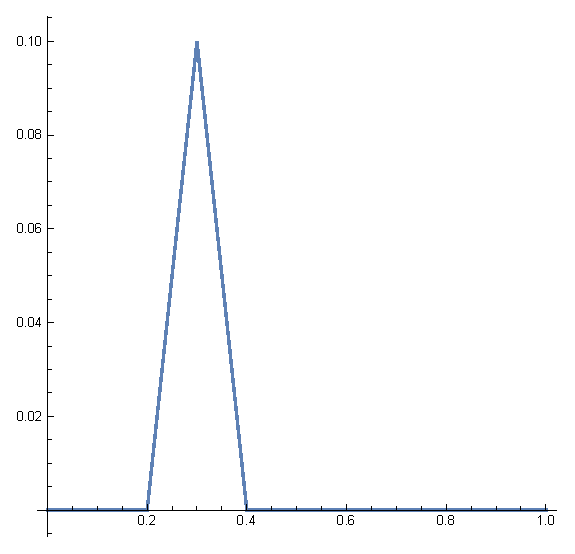
\includegraphics[width=5.5cm]{peak.eps}
\caption{A peak function where $a=0$, $b=1$, $t=0.2$, $\delta=0.1$. \label{fig:peakfunction}}
\end{figure}

Other properties of the peak function are displayed below:
\begin{gather*}
  \text{peak}'(x;t,\delta):= \begin{cases} \displaystyle 1, & t \le x < t+\delta,\\[1ex]
\displaystyle -1, & t+\delta \le x < t+2\delta,\\[1ex]
\displaystyle  0, & \text{otherwise},
\end{cases}, \\
\Var(\text{peak}'(\cdot;t,\delta))\le 4 \text{ with equality if } a<t<t+2\delta<b, \\
\int_{a}^{b}\text{peak}(x;t,\delta)dx=\delta^2.
\end{gather*}
The peak function above is continuous and with finite variation of the first derivative of the function, namely $\text{peak}(x;t,\delta)\in\cv^1$. The picture of the peak function is shown in \ref{fig:peakp1}:
\begin{figure}[ht]
\centering
\includegraphics[width=5.5cm]{peakp1.eps}
\caption{First derivative of peak function \ref{peakfunction}. \label{fig:peakp1}}
\end{figure}
Starting from this peak function $\text{peak}(x;t,\delta)$, the following double-peak functions are good candidates as fooling functions:
\begin{subequations}
    \begin{multline}\label{foolingfunctiontrap}
        \text{twopk}(x;t,\delta,\pm):=\text{peak}(x;a,\mathfrak{\delta})\pm\frac{3[\mathfrak{C}(\delta)-1]}{4}\text{peak}(x;t,\delta)\\ a+3\mathfrak{\delta}\le t \le b-3\delta, 0\le \delta <\mathfrak{h}.
    \end{multline}
    \begin{equation}
        \Var(\text{twopk}'(x;t,\delta,\pm))=3+4\frac{3[\mathfrak{C}(\delta)-1]}{4}=3\mathfrak{C}(\delta).
    \end{equation}
\end{subequations}
Picture \ref{fig:twopkfunction} shows the shape of the double-peak function $\text{twopk}(x;t,\delta,+)$.
\begin{figure}[ht]
\centering
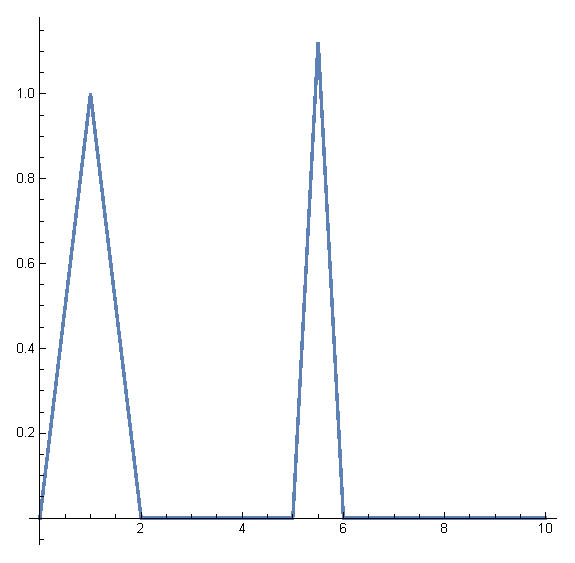
\includegraphics[width=5.5cm]{twopk.eps}
\caption{A fooling function that can fool the trapezoidal rule algorithms, where $a=0$, $b=1$, $t=0.5$, $\delta=0.05$ and $\mathfrak{h}=0.1$. \label{fig:twopkfunction}}
\end{figure}
Note that $\text{twopk}(x;t,\delta,\pm)$ are always in $\cc^1$.
From the definition of the peak function, it follows that
\begin{align*}
  &\mathfrak{C}(\text{size}(\{x_j\}_{j=0}^{n+1}))\widehat{V}(\text{twopk}'(x;t,\delta,\pm),\{x_j\}_{j=0}^{n+1})\\
  \ge & \begin{cases} \displaystyle 3\mathfrak{C}(\delta)=\Var(\text{twopk}'(x;t,\delta,\pm)), \delta \le \text{size}(\{x_j\}_{j=0}^{n+1})) <\mathfrak{h}\\[1ex]
                      \displaystyle \mathfrak{C}(0)\Var(\text{twopk}'''(x;t,\delta,\pm)), 0\le \text{size}(\{x_j\}_{j=0}^{n+1}))<\delta
        \end{cases}\\
  \ge & \Var(\text{twopk}'(x;t,\delta,\pm))
\end{align*}
The functions $\text{twopk}(x;t,\delta,\pm)$ have two peaks. The first always starts from the left end, $a$, and has the width of $2\mathfrak{h}$. The second starts from any point $t$ that is at least one interval right to the first peak and have a smaller width of $2\delta$. Although $\text{twopk}(x;t,\delta,\pm)$ may have a bump with arbitrarily small width $2\delta$, the height is small enough for $\text{twopk}(x;t,\delta,\pm)$ to lie in the cone. These two functions can be used as our fooling functions.

The fooling functions leads to the lower bound of complexity of the trapezoidal algorithm. The key to the proof is to find one appropriate $\delta$.  This $\delta$ makes the smaller peak resides within one interval of data sites. Thus the small peak cannot be detected by the algorithm. Therefore, the algorithm cannot distinguish between $\text{peak}(x;t,\delta)$ and $\text{twopk}(x;t,\delta,\pm)$. Assume that the algorithm $\texttt{int}(\cdot,\varepsilon)$ uses $n$ equally spaced nodes to successfully return and answer. Moreover, assume that $\{x_{j}\}_{j=0}^{m}$, $m<n$, is a subinterval of $\{x_{j}\}_{j=0}^{n}$ where the smaller peak resides. Notice that average width of intervals is $(x_{m+1}-x_{0})(m+1)$ and $x_{m+1}-x_{0}=b-a-3\mathfrak{h}-\delta$. Choosing one interval such that the width is less than $2\delta$, the width of small bump can make the fooling functions fool the algorithm. In order to do that, one can choose interval wider than average and $2\delta$ narrower than average.

  \begin{align*}
    \frac{x_{j+1}-x_{j}}{2}&\ge\frac{x_{m+1}-x_{0}}{2(m+1)}\ge\frac{x_{m+1}-x_{0}}{2(n+1)}=\frac{b-a-3\mathfrak{h}-\delta}{2n+2}=\delta,\\
    \Rightarrow \delta&=\frac{b-a-3\mathfrak{h}}{2n+3}
  \end{align*}

Therefore, the lower bound of the complexity for the integration problem using the trapezoidal rule can be represented as:
\begin{theorem} \label{comptrap}
Let $\texttt{int}(\cdot,\varepsilon)$ be any (possibly adaptive) algorithm that succeeds for all integrands in $\cc^1$, and only uses function values. For any error tolerance $\varepsilon > 0$ and any arbitrary value of $\Var(f')$, there will be some $f\in \cc^1$ for which $\texttt{int}(\cdot,\varepsilon)$ must use at least
    \begin{equation}\label{complowbdtrap}
        -\frac{3}{2}+\frac{b-a-3\mathfrak{h}}{4}\sqrt{\left[\frac{[\mathfrak{C}(0)-1]\Var( f')}{\varepsilon}\right]}
    \end{equation}
    function values. As $\Var(f')/\varepsilon \rightarrow \infty$ the asymptotic rate of increase is the same as the computational cost of {\tt integral\_t}. The adaptive trapezoidal {\tt integral\_t} has optimal order for integration of functions in $\cc^1$.
\end{theorem}
\begin{proof}
  For any positive $\alpha$, suppose that $\texttt{int}(\cdot,\varepsilon)$ evaluates integrand $\alpha\text{peak}'(\cdot;t,\delta)$ at $n$ nodes before returning to an answer. Let $\{x_j\}_{j=1}^{m})$ be the $m<n$ ordered nodes used by $\texttt{int}(\cdot,\varepsilon)$ that fall in the interval $(x_{0},x_{m+1})$ where $x_{0}:=a+2\mathfrak{h}$, $x_{m+1}:=b-\delta$ and $\delta:=(b-a-3\mathfrak{h})/(2n+3)$. There must exit at least one of these $x_{j}$ with $i=0,\cdots,m$ for which
  \begin{align*}
    \frac{x_{j+1}-x_{j}}{2}\ge\frac{x_{m+1}-x_{0}}{2(m+1)}\ge\frac{x_{m+1}-x_{0}}{2(n+1)}=\frac{b-a-3\mathfrak{h}-\delta}{2n+2}=\delta.
  \end{align*}
  Choose one such $x_{j}$ and call it $t$. The choice of $t$ and $\delta$ ensures that $\texttt{int}(\cdot,\varepsilon)$ cannot distinguish between $\alpha\textup{peak}(\cdot;t,\delta)$ and $\alpha\textup{twopk}(\cdot;t,\delta,\pm)$. Thus
  \begin{align*}
    \texttt{int}(\alpha\text{twopk}(\cdot;t,\delta,\pm),\varepsilon)=\texttt{int}(\alpha\text{peak}(\cdot;t,\delta),\varepsilon)
  \end{align*}
  Moreover, $\alpha\text{peak}(\cdot;t,\delta)$ and $\alpha\text{twopk}(\cdot;t,\delta,\pm)$ are all in the cone $\cc^1$. This means that $\texttt{int}(\cdot,\varepsilon)$ is successful for all of the functions.
  \begin{subequations}
  \begin{multline*}
    \varepsilon\ge\frac{1}{2}\left[\right.\left|\int_{a}^{b}\alpha\textup{twopk}(x;t,\delta,-)dx-\texttt{int}(\alpha\textup{twopk}(\cdot;t,\delta,-),\varepsilon)\right|\\
    +\left|\int_{a}^{b}\alpha\textup{twopk}(x;t,\delta,+)dx-\texttt{int}(\alpha\textup{twopk}(\cdot;t,\delta,+),\varepsilon)\right|\left.\right]
  \end{multline*}
  \begin{multline*}
    \ge\frac{1}{2}\left[\right.\left|\texttt{int}(\alpha\textup{peak}(\cdot;t,\delta,-),\varepsilon)-\int_{a}^{b}\alpha\textup{twopk}(x;t,\delta,-)dx\right|\\
    +\left|\int_{a}^{b}\alpha\textup{twopk}(x;t,\delta,+)dx-\texttt{int}(\alpha\textup{peak}(\cdot;t,\delta,+),\varepsilon)\right|\left.\right]
  \end{multline*}
  \begin{align*}
     &\ge\frac{1}{2}\left|\int_{a}^{b}\alpha\textup{twopk}(x;t,\delta,+)dx-\int_{a}^{b}\alpha\textup{twopk}(x;t,\delta,-)dx\right|\\
     &=\int_{a}^{b}\alpha\textup{peak}(x;t,\delta)dx\\
     &=\frac{3\alpha[\mathfrak{C}(\delta)-1]\delta^2}{4}\\
     &=\frac{[\mathfrak{C}(\delta)-1]\delta^2\Var(\alpha\textup{peak}'(\cdot;a,\mathfrak{h}))}{4}
  \end{align*}
  \end{subequations}
  Substituting $\delta$  in terms of $n$:
      \begin{align*}
        2n+3=\frac{b-a-3\mathfrak{h}}{\delta}&\ge(b-a-3\mathfrak{h})\left[\frac{[\mathfrak{C}(\delta)-1]\Var(\alpha \textup{peak}'(\cdot;a,\mathfrak{h})))}{4\varepsilon}\right]^{1/2},\\
        &\ge\frac{b-a-3\mathfrak{h}}{4}\left[\frac{[\mathfrak{C}(0)-1]\Var(\alpha \textup{peak}'(\cdot;a,\mathfrak{h}))}{\varepsilon}\right]^{1/2}.
    \end{align*}
    Since $\alpha$ is an arbitrary positive number, the value of $\Var(\alpha \textup{peak}'(\cdot;a,\mathfrak{h}))$ is arbitrary.

    Finally, comparing the upper bound on the computational cost of {\tt integral\_t} in \eqref{uppbndcosttrapineq} with the lower bound on the computational cost of the best algorithm in \eqref{complowbdtrap}, both of them increase as $\mathcal{O}((\Var(f')/\varepsilon))^{1/2}$ as $(\Var(f')/\varepsilon)^{1/2}\rightarrow \infty$. Thus {\tt integral\_t} is optimal.
\end{proof}

\Section{The Simpson's Rule Complexity}

To build the fooling functions for the Simpson's rule, the B-Spline expansion in the previous section continuous to the third order as follows:

\begin{align*}
  \text{b}_{j,0}(x):= \begin{cases} \displaystyle 1, & t_{j} \le x < t_{j+1},\\[1ex]
\displaystyle  0, & \text{otherwise},
\end{cases}
\end{align*}

\begin{align*}
  \text{b}_{j,1}(x):= \begin{cases} \displaystyle \frac{x-t_{j}}{t_{j+1}-t_{j}}, & t_{j} \le x < t_{j+1},\\[1ex]
\displaystyle \frac{t_{j+2}-x}{t_{j+2}-t_{j+1}}, & t_{j+1} \le x < t_{j+2},\\[1ex]
\displaystyle  0, & \text{otherwise},
\end{cases}
\end{align*}

\begin{align*}
  \text{b}_{j,2}(x):= \begin{cases} \displaystyle \frac{(x-t_{j})^2}{2(t_{j+1}-t_{j})^2}, & t_{j} \le x < t_{j+1},\\[1ex]
\displaystyle \frac{(t_{j+2}-x)(x-t_{j})}{2(t_{j+2}-t_{j+1})^2}+\frac{(t_{j+3}-x)(x-t_{j+2})}{2(t_{j+2}t_{j+1})^2}, & t_{j+1} \le x < t_{j+2},\\[1ex]
\displaystyle \frac{(t_{j+3}-x)^2}{2(t_{j+3}-t_{j+2})^2}, & t_{j+2} \le x < t_{j+3},\\[1ex]
\displaystyle  0, & \text{otherwise},
\end{cases}
\end{align*}

\begin{align*}
  \text{b}_{j,3}(x):= \begin{cases} \displaystyle \frac{(x-t_{j})^3}{6(t_{j+1}-t_{j})^3}, & t_{j} \le x < t_{j+1},\\[1ex]
\displaystyle \frac{(t_{j+2}-x)(x-t_{j})^2}{6(t_{j+2}-t_{j+1})^3}+\frac{(t_{j+3}-x)(x-t_{j})(x-t_{j+1})}{6(t_{j+2}-t_{j+1})^3}\\[1ex]\displaystyle\quad+\frac{(t_{j+4}-x)(x-t_{j+1})^2}{6(t_{j+2}-t_{j+1})^3},& t_{j+1} \le x < t_{j+2},\\[1ex]
\displaystyle \frac{(t_{j+3}-x)^2(x-t_{j})}{6(t_{j+3}-t_{j+2})^3}+\frac{(t_{j+4}-x)(t_{j+3}-x)(x-t_{j+1})}{6(t_{j+3}-t_{j+2})^3}\\[1ex]\displaystyle\quad+\frac{(t_{j+4}-x)^2(x-t_{j+2})}{6(t_{j+3}-t_{j+2})^3},& t_{j+2} \le x < t_{j+3},\\[1ex]
\displaystyle \frac{(t_{j+4}-x)^3}{6(t_{j+4}-t_{j+3})^3}, & t_{j+3} \le x < t_{j+4},\\[1ex]
\displaystyle  0, & \text{otherwise},
\end{cases}
\end{align*}

%\begin{align*}
%  \text{b}_{j,3}(x):= \begin{cases} \displaystyle \frac{(x-t_{j})^3}{6h^3}, t_{j} \le x < t_{j+1},\\[10ex]
%\displaystyle \frac{(t_{j+2}-x)(x-t_{j})^2}{6h^3}+\frac{(t_{j+3}-x)(x-t_{j})(x-t_{j+1})}{6h^3}+\frac{(t_{j+4}-x)(x-t_{j+1})^2}{6h^3}, \\[1ex]
%\displaystyle \frac{(t_{j+3}-x)^2(x-t_{j})}{6h^3}+\frac{(t_{j+4}-x)(t_{j+3}-x)(x-t_{j+1})}{6h^3}+\frac{(t_{j+4}-x)^2(x-t_{j+2})}{6h^3}, \\[1ex]
%\displaystyle \frac{(t_{j+4}-x)^3}{6h^3}, t_{j+3} \le x < t_{j+4},\\[1ex]
%\displaystyle  0, \text{otherwise},
%\end{cases}
%\end{align*}

%\begin{align*}
%  \text{b}_{j,3}'''(x):= \begin{cases} \displaystyle 1/h^3, & t_{j} \le x < t_{j+1},\\[1ex]
%\displaystyle -3/h^3, & t_{j+1} \le x < t_{j+2},\\[1ex]
%\displaystyle 3/h^3, & t_{j+2} \le x < t_{j+3},\\[1ex]
%\displaystyle -1/h^3, & t_{j+3} \le x < t_{j+4},\\[1ex]
%\displaystyle  0, & \text{otherwise},
%\end{cases},
%\end{align*}
The function $\text{b}_{j,3}(x)$ is a bump shaped function that starts at point $t_j$, with the width of $t_{j+4}-t_{j}$ and zero value elsewhere than $(t_{j}, t_{j+4})$. Assuming that $\{t_{j}\}_{j=1}^{n}$ is equally space between $(a,b)$, $t_{j+1}-t_{j}=\delta$, and $t=t_{j}$ . The bump function is defined as

%\begin{gather}
%bump(x;t,h):= \begin{cases} \displaystyle (x-t)^3/6, & t \le x < t+h,\\[1ex]
%\displaystyle [(x-t)^2(t+2h-x)+(x-t)(t+3h-x)(x-t-h)+(t+4h-x)(x-t-h)^2]/6, & t+h \le x < t+2h,\\[1ex]
%\displaystyle [(x-t)(t+3h-x)^2+(t+4h-x)(x-t-h)(t+3h-x)+(t+4h-x)^2(x-t-2h)]/6, & t+2h \le x < t+3h,\\[1ex]
%\displaystyle (t+4h-x)^3/6, & t+3h \le x < t+4h,\\[1ex]
%\displaystyle  0, & \text{otherwise},
%\end{cases}
%\\
\begin{align} \label{bumpfunction}
\text{bump}(x;t,h):= \begin{cases} \displaystyle (x-t)^3/6,  &t \le x < t+\delta,\\[1ex]
\displaystyle [-3(x-t)^3+12\delta(x-t)^2\\[1ex] \displaystyle\qquad -12\delta^2(x-t)+4\delta^3]/6,  &t+\delta \le x < t+2\delta,\\[1ex]
\displaystyle [3(x-t)^3-24\delta(x-t)^2\\[1ex]  \displaystyle\qquad +60\delta^2(x-t)-44\delta^3]/6, &t+2\delta \le x < t+3\delta,\\[1ex]
\displaystyle (t+4\delta-x)^3/6,  &t+3\delta \le x < t+4\delta,\\[1ex]
\displaystyle  0,  &\text{otherwise},
\end{cases}
\end{align}
Picture \ref{fig:bumpfunction} shows the shape of the bump function. The bump function is continuous.
\begin{figure}[ht]
\centering
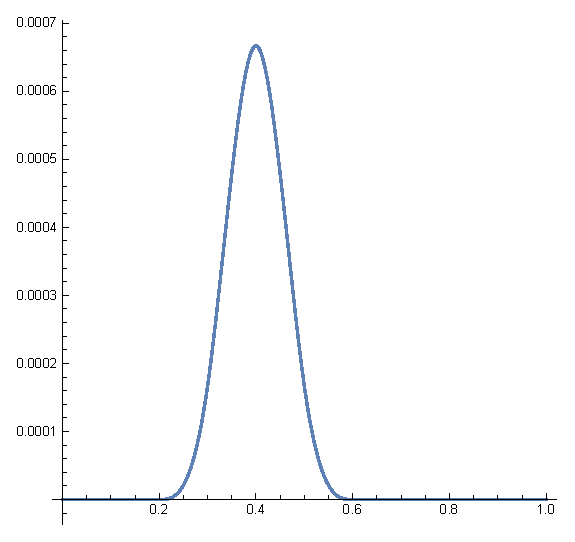
\includegraphics[width=5.5cm]{bump.eps}
\caption{A bump function, where $a=0$, $b=1$, $t=0.2$, $\delta=0.1$ and $\mathfrak{h}=0.1$. \label{fig:bumpfunction}}
\end{figure}

Other properties of the bump function are displayed below.
\begin{subequations}
\begin{gather}
\text{bump}'(x;t,\delta):= \begin{cases} \displaystyle (x-t)^{2}/2, & t \le x < t+\delta,\\[1ex]
\displaystyle -[3(x-t)^{2}-8\delta(x-t)+4\delta^2]/2, & t+\delta \le x < t+2\delta,\\[1ex]
\displaystyle [3(x-t)^{2}-16\delta(x-t)+20\delta^2]/2, & t+2\delta \le x < t+3\delta,\\[1ex]
\displaystyle -(x-t-4\delta)^2/2, & t+3\delta \le x < t+4\delta,\\[1ex]
\displaystyle  0, & \text{otherwise},
\end{cases}, \\
\text{bump}''(x;t,\delta):= \begin{cases} \displaystyle (x-t), & t \le x < t+\delta,\\[1ex]
\displaystyle -3(x-t)+4\delta, & t+\delta \le x < t+2\delta,\\[1ex]
\displaystyle 3(x-t)-8\delta, & t+2\delta \le x < t+3\delta,\\[1ex]
\displaystyle -(x-t-4\delta), & t+3\delta \le x < t+4\delta,\\[1ex]
\displaystyle  0, & \text{otherwise},
\end{cases}, \\
\text{bump}'''(x;t,\delta):= \begin{cases} \displaystyle 1, & t \le x < t+\delta,\\[1ex]
\displaystyle -3, & t+\delta \le x < t+2\delta,\\[1ex]
\displaystyle 3, & t+2\delta \le x < t+3\delta,\\[1ex]
\displaystyle -1, & t+3\delta \le x < t+4\delta,\\[1ex]
\displaystyle  0, & \text{otherwise},
\end{cases}, \\
\Var(\text{bump}'''(\cdot;t,\delta))\le 16 \text{ with equality if } a<t<t+4\delta<b, \\
\int_{a}^{b}\text{bump}(x;t,\delta)dx=\delta^4.
\end{gather}
\end{subequations}
\begin{figure}[ht]
\centering
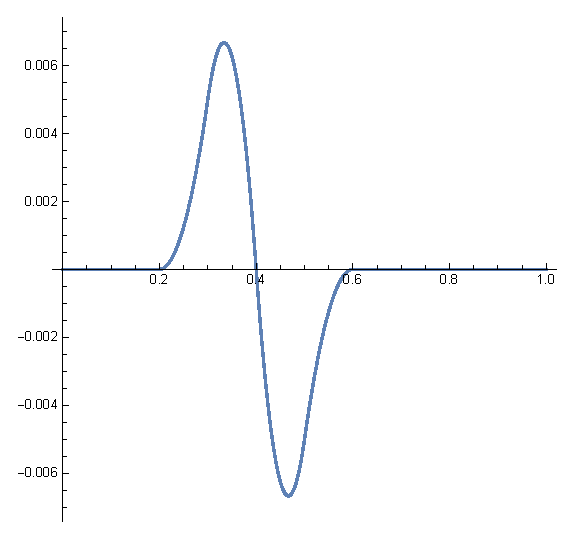
\includegraphics[width=5.5cm]{bumpp1.eps}
\caption{First derivative of bump function \ref{fig:bumpfunction}. \label{fig:bumpp1}}
\end{figure}
\begin{figure}[ht]
\centering
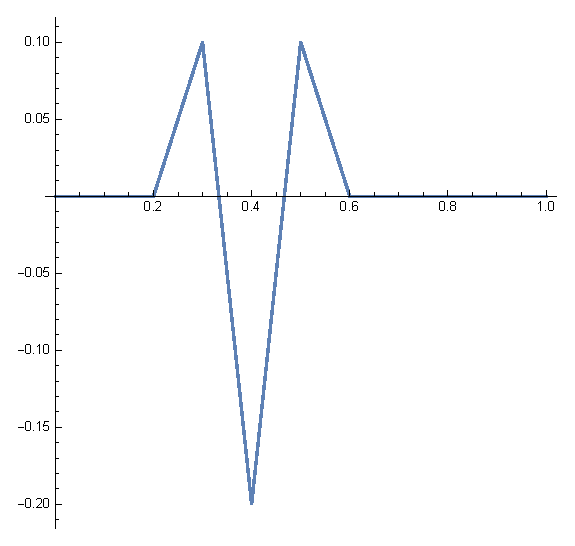
\includegraphics[width=5.5cm]{bumpp2.eps}
\caption{Second derivative of bump function \ref{fig:bumpfunction}. \label{fig:bumpp2}}
\end{figure}
\begin{figure}[ht]
\centering
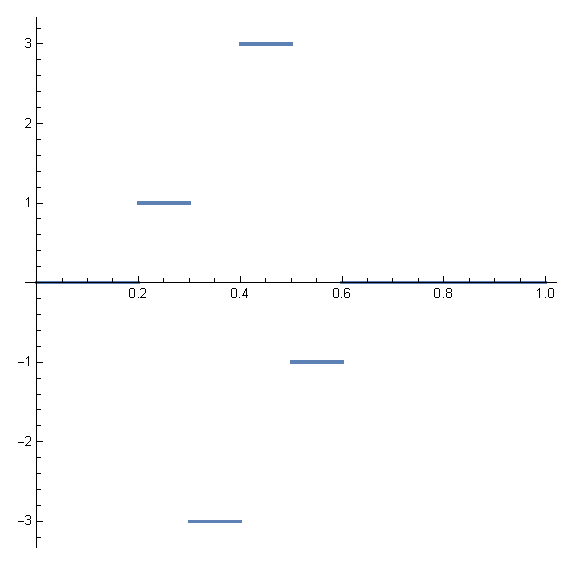
\includegraphics[width=5.5cm]{bumpp3.eps}
\caption{Third derivative of bump function \ref{fig:bumpfunction}. \label{fig:bumpp3}}
\end{figure}
The bump function above is continuous to the third derivative with finite variation of the third derivatives. Note that the following double-bump function that is always in $\cc^3$:
\begin{subequations}
    \begin{multline}\label{foolingfunctionsim}
        \text{twobp}(x;t,\delta,\pm):=\text{bump}(x;a,\mathfrak{h})\pm\frac{15[\mathfrak{C}(\delta)-1]}{16}\text{bump}(x;t,\delta)\\ a+5\mathfrak{h}\le x \le b-5\delta, 0\le \delta <\mathfrak{h}.
    \end{multline}
    \begin{equation}
        \Var(\text{twobp}'''(x;t,\delta,\pm))=15+16\frac{15[\mathfrak{C}(\delta)-1]}{16}=15\mathfrak{C}(\delta).
    \end{equation}
\end{subequations}
Picture \ref{fig:twobpfunction} shows the shape of the double-peak function.
\begin{figure}[ht]
\centering
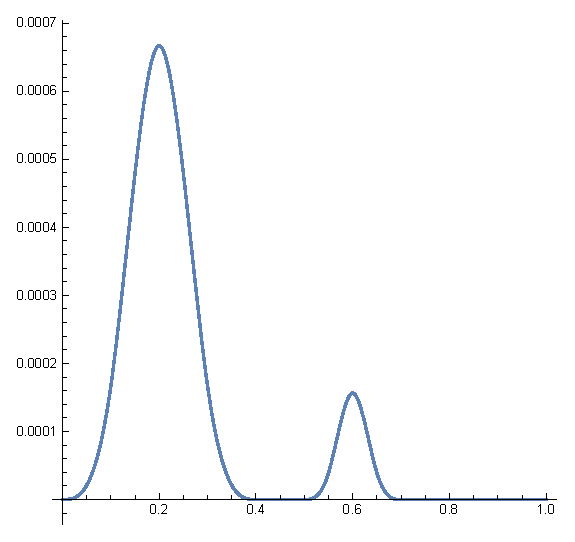
\includegraphics[width=5.5cm]{twobp.eps}
\caption{A fooling function that can fool the Simpson's rule algorithms, where $a=0$, $b=1$, $t=0.5$, $\delta=0.05$ and $\mathfrak{h}=0.1$. \label{fig:twobpfunction}}
\end{figure}

From this properties of the bump function, it follows that
\begin{align*}
  &\mathfrak{C}(\text{size}(\{x_j\}_{j=0}^{n+1}))\widehat{V}(\text{twobp}'''(x;t,\delta,\pm),\{x_j\}_{j=0}^{n+1})\\
  \ge & \begin{cases} \displaystyle 15\mathfrak{C}(\delta)=\Var(\text{twobp}'''(x;t,\delta,\pm)), \delta \le \text{size}(\{x_j\}_{j=0}^{n+1})) <\mathfrak{h}\\[1ex]
                      \displaystyle \mathfrak{C}(0)\Var(\text{twobp}'''(x;t,\delta,\pm)), 0\le \text{size}(\{x_j\}_{j=0}^{n+1}))<\delta
        \end{cases}\\
  \ge & \Var(\text{twobp}'''(x;t,\delta,\pm))
\end{align*}
Although $\text{twobp}'''(x;t,\delta,\pm)$ may have a bump with arbitrarily small width $4\delta$, the height is small enough for $\text{twobp}'''(x;t,\delta,\pm)$ to lie in the cone.

Similar to the trapezoidal case, the average width of intervals is $(x_{m+1}-x_{0})/(m+1)$ and $x_{m+1}-x_{0}=b-a-5\mathfrak{h}-\delta$. Choose one interval such that width less bigger than $4\delta$ (the width of small bump). In order to do that, we can choose interval wider than average and $4\delta$ narrower than average:
  \begin{align*}
    \frac{x_{j+1}-x_{j}}{4}&\ge\frac{x_{m+1}-x_{0}}{4(m+1)}\ge\frac{x_{m+1}-x_{0}}{4(n+1)}=\frac{b-a-5\mathfrak{h}-\delta}{4n+4}=\delta,\\
    \Rightarrow \delta&=\frac{b-a-5\mathfrak{h}}{4n+5}
  \end{align*}

With the fooling functions, the lower bound of complexity of the Simpson's algorithms can be expressed as follow.
\begin{theorem}\label{compsim}
    Let $\texttt{int}$ be any (possibly adaptive) algorithm that succeeds for all integrands in $\cc^3$, and only uses integrand values. For any error tolerance $\varepsilon > 0$ and any arbitrary value of $\Var(f''')$, there will be some $f\in \cc^3$ for which $\texttt{int}$ must use at least
    \begin{equation}\label{complowbdsim}
        -\frac{5}{4}+\frac{b-a-5\mathfrak{h}}{8}\left[\frac{[\mathfrak{C}(0)-1]\Var( f''')}{\varepsilon}\right]^{1/4}
    \end{equation}
    function values. As $\Var(f''')/\varepsilon \rightarrow \infty$ the asymptotic rate of increase is the same as the computational cost of {\tt integral\_s}. Thus {\tt integral\_s} has optimal order for integration of functions in $\cc^3$.
\end{theorem}
\begin{proof}
  For any positive $\alpha$, suppose that $\texttt{int}(\cdot,\varepsilon)$ evaluates integrand $\alpha\text{bump}'''(\cdot;t,\delta)$ at $n$ nodes before returning to an answer. Let $\{x_j\}_{j=1}^{m})$ be the $m<n$ ordered nodes used by $\texttt{int}(\cdot,\varepsilon)$ that fall in the interval $(x_{0},x_{m+1})$ where $x_{0}:=a+3\mathfrak{h}$, $x_{m+1}:=b-\delta$ and $\delta:=(b-a-5\mathfrak{h})/(4n+5)$. There must exits at least one of these $x_{j}$ with $i=0,\cdots,m$ for which
  \begin{align*}
    \frac{x_{j+1}-x_{j}}{4}\ge\frac{x_{m+1}-x_{0}}{4(m+1)}\ge\frac{x_{m+1}-x_{0}}{4(n+1)}=\frac{b-a-5\mathfrak{h}-\delta}{4n+4}=\delta.
  \end{align*}
  Choose one such $x_{j}$ and call it $t$. The choice of $t$ and $\delta$ ensures that $\texttt{int}(\cdot,\varepsilon)$ cannot distinguish between $\alpha\text{bump}(\cdot;t,\delta)$ and $\alpha\text{twobp}(\cdot;t,\delta,\pm)$. Thus
  \begin{align*}
    \texttt{int}(\alpha\text{twobp}(\cdot;t,\delta,\pm),\varepsilon)=\texttt{int}(\alpha\text{bump}(\cdot;t,\delta),\varepsilon)
  \end{align*}
  Moreover, $\alpha\textup{bump}(\cdot;t,\delta)$ and $\alpha\textup{twobp}(\cdot;t,\delta,\pm)$ are all in the cone $\cc^3$. This means that $\texttt{int}(\cdot,\varepsilon)$ is successful for all of the functions.
  \begin{subequations}
  \begin{multline*}
    \varepsilon\ge\frac{1}{2}\left[\right.\left|\int_{a}^{b}\alpha\textup{twobp}(x;t,\delta,-)dx-\texttt{int}(\alpha\textup{twobp}(\cdot;t,\delta,-),\varepsilon)\right|\\
    +\left|\int_{a}^{b}\alpha\textup{twobp}(x;t,\delta,+)dx-\texttt{int}(\alpha\textup{twobp}(\cdot;t,\delta,+),\varepsilon)\right|\left.\right]
  \end{multline*}
  \begin{multline*}
    \ge\frac{1}{2}\left[\right.\left|\texttt{int}(\alpha\textup{bump}(\cdot;t,\delta,-),\varepsilon)-\int_{a}^{b}\alpha\textup{twobp}(x;t,\delta,-)dx\right|\\
    +\left|\int_{a}^{b}\alpha\textup{twobp}(x;t,\delta,+)dx-\texttt{int}(\alpha\textup{bump}(\cdot;t,\delta,+),\varepsilon)\right|\left.\right]
  \end{multline*}
  \begin{align*}
     &\ge\frac{1}{2}\left|\int_{a}^{b}\alpha\textup{twobp}(x;t,\delta,+)dx-\int_{a}^{b}\alpha\textup{twobp}(x;t,\delta,-)dx\right|\\
     &=\int_{a}^{b}\alpha\textup{bump}(x;t,\delta)dx\\
     &=\frac{15\alpha[\mathfrak{C}(\delta)-1]\delta^4}{16}\\
     &=\frac{[\mathfrak{C}(\delta)-1]\delta^4\Var(\alpha\textup{bump}'''(\cdot;a,\mathfrak{h}))}{16}
  \end{align*}
  \end{subequations}
  Substituting $\delta$  in terms of $n$:
      \begin{align*}
        4n+5=\frac{b-a-5\mathfrak{h}}{\delta}&\ge(b-a-5\mathfrak{h})\left[\frac{[\mathfrak{C}(\delta)-1]\Var(\alpha \textup{bump}'''(\cdot;a,\mathfrak{h})))}{16\varepsilon}\right]^{1/4},\\
        &\ge-\frac{5}{4}+\frac{b-a-5\mathfrak{h}}{8}\left[\frac{[\mathfrak{C}(0)-1]\Var(\alpha \textup{bump}'''(\cdot;a,\mathfrak{h}))}{\varepsilon}\right]^{1/4}.
    \end{align*}
    Since $\alpha$ is an arbitrary positive number, the value of $\Var(\alpha \texttt{bump}'''(\cdot;a,\mathfrak{h}))$ is arbitrary.

    Finally, comparing the upper bound on the computational cost of {\tt integral\_s} in \eqref{uppbndcostineqsim} with the lower bound on the computational cost of the best algorithm in \eqref{complowbdsim}, both of them increase as $\mathcal{O}((\Var(f''')/\varepsilon))^{1/4}$ as $(\Var(f''')/\varepsilon)^{1/4}\rightarrow \infty$. Thus {\tt integral\_s} is optimal.
\end{proof}

Having proved that our algorithms using the trapezoidal rule and Simpson's rule are optimal, the author continuous to test the performance of the two algorithms. In the next chapter, the numerical results from {\tt integral\_t} and {\tt integral\_s} are discussed.

\Chapter{Numerical Experiments}

The bump function $\text{bump}(x;t,\delta)$ defined in \eqref{bumpfunction} is used as our test function to check the performance of our algorithms. Consider the family of bump test functions on interval $(0,1)$ defined by
\begin{equation}\label{testfun}
f(x,t,\delta)= \text{bump}(x;t,\delta)/\delta^{4}
\end{equation}
with  $t \sim \cu[0,1-4\delta]$, $\log_{10}(\delta) \sim \cu[-4,-1]$. The integration $\int_{0}^{1}f(x,t,\delta)\text{d}x=1$. Input $t$ controls the starting position of the bump. The starting point is randomly chosen between $0$ and $1-4\delta$. Input $\delta$ controls the quarter width of the bump. The random quarter width expands from $0.0001$ to $0.1$.
%It follows that $\norm[1]{f'-f(1)+f(0)}=1/a$ and $\Var(f')=2/a^2$.  The probability that $f \in \cc_{\tau}$ is $\min\left(1,\max(0,\left(\log_{10}(\tau/2)-1\right)/3)\right).$
As an experiment, we chose $10000$ random test functions and applied {\tt integral\_t} and {\tt integral\_s} with an error tolerance of  $\varepsilon = 10^{-8}$. The initial values of $\mathfrak{h}$ are set as $0.1$, $0.01$, and $0.001$. The algorithm is considered successful for a particular $f$ if the exact and approximate integrals have a difference no greater than $\varepsilon$. Our algorithms give warnings when the integrand is not in the original cone. The success rates are given in Table \ref{integresultstable}. %Our algorithm imposes a cost budget of $N_{\max}=10^7$.
%If the proposed $n_{i+1}$ in Stages 2 or 3 exceeds $N_{\max}$, then our algorithm returns a warning and falls back to the largest possible $n_{i+1}$ not exceeding $N_{\max}$ for which $n_{i+1}-1$ is a multiple of $n_i-1$.  The probability that $f$ initially lies in $\cc_{\tau}$ is the smaller number in the third column of Table \ref{integresultstable}, while the larger number is the empirical probability that $f$ eventually lies in $\cc_{\tau}$ after possible increases in $\tau$ made by Stage 2 of Algorithm \ref{multistageintegalgo}.  For this experiment Algorithm \ref{multistageintegalgo} was successful for all $f$ that finally lie inside $\cc_{\tau}$ and for which no attempt was made to exceed the cost budget.

%\begin{table}[h]
%\centering
%\begin{tabular}{cccccc}
%&&&Success & Success & Failure \\
%& $\tau$ &  $\Prob(f \in \cc_{\tau}) $ & No Warning & Warning & No Warning \\
%\toprule
%&$10$ & $0\% \rightarrow  25\% $ & $25\%$ & $<1\%$ & $75\%$  \\
%Algorithm \ref{multistagetrapalgo}
% &$100$ & $23 \% \rightarrow 58\% $ & $56\%$ & $2\%$ & $42\%$ \\
%&$1000$ & $57\% \rightarrow 88\% $& $68\%$ & $20\%$ &$12\%$ \\
%\midrule
%{\tt quad} & & & 8\% & & $92\%$\\
%{\tt integral} & & & 19\% & & $81\%$\\
%{\tt chebfun} & & &29\% & & $71\%$\\
%\end{tabular}
%\caption{The probability of the test function lying in the cone for the original and eventual values of $\tau$ and the empirical success rate of Algorithm \ref{multistagetrapalgo} and Algorithm \ref{multistageintegalgosimpson} plus the success rates of other common quadrature algorithms. \label{integresultstable}}
%\end{table}
\begin{table}[ht]
\caption{The success rates of {\tt integral\_t} and {\tt integral\_s} plus the success rates of other common quadrature algorithms.}
\centering
\begin{tabular}{cccc}
\hline\hline
& $\mathfrak{h}$ & Success & Success Warning \\
\hline
&$0.1$  & $24.76\%$ &  $9.43\%$  \\
{\tt integral\_t}
 &$0.01$  & $57.36\%$ & $3.70\%$ \\
&$0.001$ & $87.38\%$ &$0.81\%$ \\
\hline
&$0.1$  & $25.94\%$ &  $14.28\%$  \\
{\tt integral\_s}
 &$0.01$  & $57.63\%$ & $4.45\%$ \\
&$0.001$ & $94.09\%$ &$0.87\%$ \\
\hline
{\tt integral} & & 29.68 \% & \\
{\tt chebfun} & &18.91\% & \\
\hline
\end{tabular}
\label{integresultstable}
\end{table}

Some commonly available numerical algorithms in MATLAB are {\tt integral} \cite{MAT8.1} and the MATLAB Chebfun toolbox \cite{TrefEtal12}. We applied these two routines to the random family of test functions as well.  Their success and failure rates are also recorded in Table \ref{integresultstable}.  They do not give warnings of possible failure.

%\Section{Simpson's Rule}
%\textcolor{red}{I need to use a good example to run the tests. Then I will need to compare the results for both algorithms with other algorithms. After that, I need to compare trap and sim to get the conclusion such as sim has faster convergence rate than trap. This will require an sample function good to both trap and sim.}
The test results in Table \ref{integresultstable} shows that both {\tt integral\_t} and {\tt integral\_s} return higher success rates as the initial cut-off value $\mathfrak{h}$ being smaller. This makes sense because higher cut-off value provides more inclusive cones. The chance of a bump function lie in the cone is higher. Thus the algorithms can guarantee to solve spikier integrands.  Both {\tt integral\_t} and {\tt integral\_s} outperform {\tt integral} and Chebfun toolbox since the fact that the test functions are defined in order to fool the algorithm. Our algorithms has the mechanism of changing $\mathfrak{h}$ to enhance the success rate. The two comparing algorithms do not have similar settings.

Convergence rate for both algorithms are also important to study. We use the test function $f(x,t,\delta)= \text{bump}(x;t,\delta)/\delta^{4}$ where $t=0.2$; $\delta=0.1$. Both {\tt integral\_t} and {\tt integral\_s} use $\mathfrak{h}=0.1$. The following picture shows the convergence rate for the two algorithms.
\begin{figure}[ht]
\centering
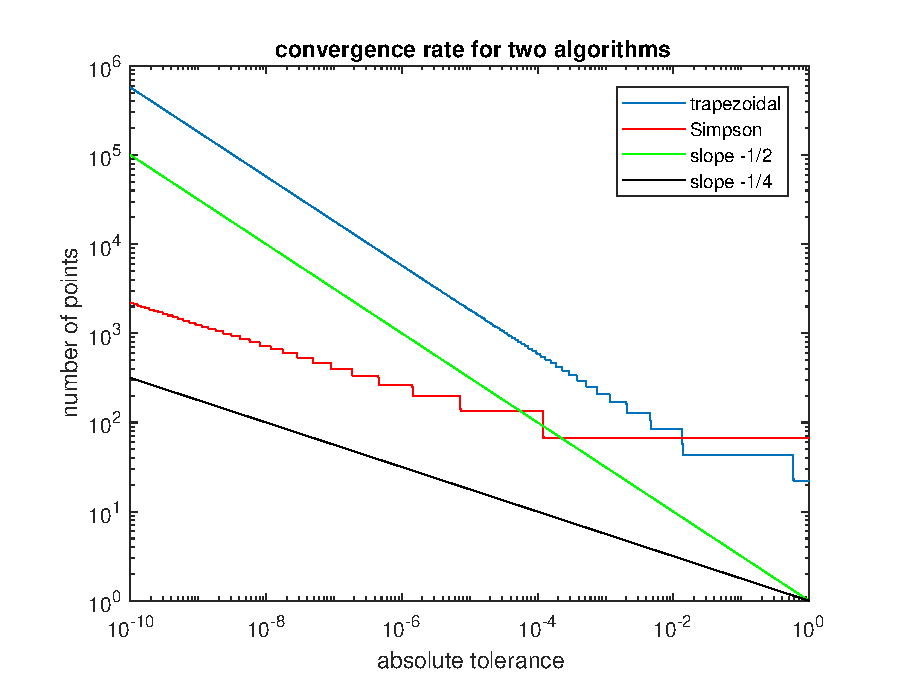
\includegraphics[width=12.5cm]{converwithslope.eps}
\caption{The convergence curves for {\tt integral\_t} and {\tt integral\_s}. \label{fig:convergencerate}}
\end{figure}

From the picture we can see that {\tt integral\_s} converges faster than {\tt integral\_t}. Moreover, {\tt integral\_t} converges at the rate of $-1/2$ to the logarithm. And {\tt integral\_s} converges at the rate of $-1/4$ to the logarithm. The results coincide with the results of the upper bound on the computational cost.


\Chapter{CONCLUSION}
 %   \input{Conclusion.tex}

In this thesis, we study the algorithms for univariate integration problems. Both algorithms using the trapezoidal rule and Simpson's rule are constructed. The approximation error for them are analyzed in terms of function values. The computational cost of the algorithms is studied in the sense of lower and upper bound of function value required for a specific error tolerance. The complexity of any algorithms using the trapezoidal rule and Simpson's rule are derived. This chapter summarizes the main results and brings out the future work to be pursued.


\Section{Summary}

Numerical approximation motivated by univariate integration problems can be categorized into two typical types. The first category is fixed-cost algorithms with guarantees. These algorithms are automatic but not adaptive since the computational cost does not depend on the integrand. The second category is adaptive, automatic algorithms such as MATLAB's integral and Chebfun. These algorithms do not have rigorous justification. The user does not know whether the returned results from the algorithm is true or not. This thesis proposed two algorithms, using the trapezoidal rule and Simpson's rule respectively, where the integrands lie in cone $\cv^1$ and $\cv^3$. For the trapezoidal rule, $\cv^{1}:=\{f\in C^{1}[a,b]: \Var(f') < \infty \}$ and the function space is
\begin{multline*}
\cc^{1}:=\left\{f\in \cv^{1}, \Var(f')\leq \mathfrak{C}(\text{size}(\{x_i\}_{i=0}^{n+1}))\widehat{V}(f',\{x_i\}_{i=0}^{n+1}),\right.\\ \left.\text{for all choices of } n\in \mathbb{N}, \text{and }\{x_i\}_{i=0}^{n+1} \text{ with }\text{size}(\{x_i\}_{i=0}^{n+1})<\mathfrak{h}\right\}.
\end{multline*}
 For the Simpson's rule, $\cv^{3}:=\{f\in C^{3}[a,b]: \Var(f''') < \infty \}$ and the function space is
 \begin{multline*}
\cc^{3}:=\left\{f\in \cv^{3}, \Var(f''')\leq \mathfrak{C}(\text{size}(\{x_i\}_{i=0}^{n+1}))\widehat{V}(f''',\{x_i\}_{i=0}^{n+1}),\right.\\ \left.\text{for all choices of } n\in \mathbb{N}, \text{and }\{x_i\}_{i=0}^{n+1} \text{ with }\text{size}(\{x_i\}_{i=0}^{n+1})<\mathfrak{h}\right\}.
\end{multline*}
  Using backward finite difference, the error estimate of the trapezoidal rule, $\overline{\textup{err}}_{\textup{t}}(f,n)$, can be bounded as follows using function values.
 \begin{equation*}
   \overline{\textup{err}}_{\textup{t}}(f,n)\leq \frac{(b-a)^2\mathfrak{C}(2(b-a)/n)\widetilde{V}_1(f,n)}{8n^2}.
 \end{equation*}
The error estimate of the Simpson's rule, $\overline{\textup{err}}_{\textup{s}}(f,n)$, can be bounded as follows using function values.
\begin{equation*}
  \overline{\textup{err}}_{\text{s}}(f,n)\leq \frac{(b-a)^4\mathfrak{C}((b-a)/n)\widetilde{V}_3(f,n)}{93312n^4}.
\end{equation*}

Detailed processes of the two new algorithms are provided. The two algorithm are proven to be successful if the integrand lies into the appropriate cone. The computational cost of the trapezoidal algorithm has lower and upper bound as
\begin{multline*}\\
        \max\left(\left\lfloor\frac{2(b-a)}{\mathfrak{h}}\right\rfloor,\left\lceil2(b-a)\sqrt{\frac{\Var(f')}{8\varepsilon}}\right\rceil\right)\leq N(f,\varepsilon)\\ \leq 2\min\left\{n\in\mathbb{N}:n\geq\left(\left\lfloor\frac{2(b-a)}{\mathfrak{h}}\right\rfloor\right),\zeta(n)\Var(f')\leq\varepsilon\right\}\\ \leq 2\min_{0<\alpha\leq1}\max\left(\left(\left\lfloor\frac{2(b-a)}{\alpha\mathfrak{h}}\right\rfloor\right),(b-a)\sqrt{\frac{\mathfrak{C}(\alpha\mathfrak{h})\Var(f')}{8\varepsilon}}\right),
    \end{multline*}
    where $\zeta(n)=(b-a)^2\mathfrak{C}(2(b-a)/n)/(8\varepsilon n^2)$. The number of function values, namely, the computational cost required by the algorithm, is $N(f,\varepsilon)+1$.
    The computational cost of the Simpson's algorithm has lower and upper bound as
    \begin{multline*}\\
         \max\left(\left\lfloor\frac{(b-a)}{\mathfrak{h}}\right\rfloor,\left\lceil(b-a)\left(\frac{\Var(f''')}{93312\varepsilon}\right)^{1/4}\right\rceil\right)\leq N(f,\varepsilon)\\ \leq 2\min\left\{n\in\mathbb{N}:n\geq\left(\left\lfloor\frac{(b-a)}{\mathfrak{h}}\right\rfloor\right),\zeta(n)\Var(f''')\leq\varepsilon\right\}\\ \leq 2\min_{0<\alpha\leq1}\max\left(\left(\left\lfloor\frac{(b-a)}{\alpha\mathfrak{h}}\right\rfloor\right),(b-a)\left(\frac{\mathfrak{C}(\alpha\mathfrak{h})\Var(f''')}{93312\varepsilon}\right)^{1/4}\right),
    \end{multline*}
  where $\zeta(n)=(b-a)^4\mathfrak{C}((b-a)/n)/(93312n^4)$. The number of function values, namely the computational cost, required by the algorithm is $6N(f,\varepsilon)+1$.

The lower bounds on the complexity for any algorithms using the trapezoidal rule and Simpson's rule are studied by constructing fooling functions. For the trapezoidal rule, the complexity has a lower bound of
$$
     -\frac{3}{2}+\frac{b-a-3\mathfrak{h}}{8}\sqrt{\left[\frac{[\mathfrak{C}(0)-1]\Var( f')}{\varepsilon}\right]}.
$$
For the Simpson's rule, the complexity has a lower bound of
$$
     -\frac{5}{4}+\frac{b-a-5\mathfrak{h}}{8}\left[\frac{[\mathfrak{C}(0)-1]\Var( f''')}{\varepsilon}\right]^{1/4}.
$$
The upper bounds of algorithms using the trapezoidal rule and Simpson's rule is asymptotically to the same order of the complexity of the problem, respectively. It is shown that our algorithms are optimal.

Results from numerical experiments of testing a family of bump functions in $\cv^3$ show that the Simpson's rule algorithm has better success rate than the trapezoidal rule algorithm. Both algorithms has better success rate than MATLAB's {\tt integral} and Chebfun. Results also show that the Simpson's rule algorithm has faster convergence rate than the trapezoidal rule algorithm.

\Section{Future Work}

Our new algorithms are designed to solve the univariate integration problems. The algorithms use the trapezoidal rule and Simpson's rule and are globally adaptive. For future work, new methods can be proposed to solve multivariate integration problems. The input points can be locally adaptive, where additional points are only added to the necessary locations according to the shape of the integrand. Making the algorithms locally adaptive may significantly save the computational cost. The error implemented in the derivations and algorithms is the absolute error. Relative error may provide more stable results when the integral is very small and be worthy to study. The convergence rates of the trapezoidal rule and Simpson's rule are not fast enough. New algorithms can be created using methods with faster convergence rate.



\clearpage


%
% APPENDIX
%%
%
%% Do the settings of appendices with \appendix command
%\appendix
%
%% Then create each appendix using
%% \Appendix{title_of_appendix} command
%
%\Appendix{Table of Transition Coefficients for the Design of
%Linear-Phase FIR Filters}
%
%Your Appendix will go here !
%
%% \moretox
%
%  \Appendix{Name of your Second
%Appendix}
%
%Your second appendix text....
%
%\Appendix{Name of your Third Appendix}
%
%Your third appendix text....
%
% BIBLIOGRAPHY
%
% you have two options: 1) create bibliography manually,
% 2) create bibliography automatically. See BibliographyHelp.pdf file for details.

%
\bibliographystyle{plain}
\bibliography{mybib}

\end{document}  % end of document
